\chapter{Results}
This chapter aims to present the results to the reader.
We tested four mechanisms for their utility and privacy, as indicated in the methodology.
For all four mechanisms, we applied a prefix to indicate the number of dimensions on which the mechanism was used.
For example, we named the piecewise mechanism used on 2-dimensional data as "2d-piecewise," even though the underlying method is not different from the original piecewise method.
The results are presented in the following order:
\begin{enumerate}
    \item Cluster utility: We use external validation (AMI/ARI) to show the difference between the three different cluster algorithms when trained privately with nD-laplace (\ref{fig:final-mechanism-design}) and piecewise.
    \item Mechanism utility: We compare the three types of laplace (normal, grid-based, and optimal truncation) and piecewise using external validation.
    \item Privacy: We compare the three types of laplace and piecewise using the ROC-curve for evaluating the membership inference attack (MIA).
    \item Dimensionality: We evaluate the influence of the number of dimensions on both utility and privacy. \todo[inline]{In progress}
    \item Shape: The shape of the data is being investigated to measure its impact on the utility and privacy of the Laplace mechanism. \todo[inline]{In progress}
\end{enumerate}
The seconts 1 till 3 are structured according to the amount of dimensions. So we start with 2-dimensional data (2D-Laplace), then 3-dimensional data (3D-Laplace), and finally n-dimensional data (nD-Laplace). See the mechanism flowchart for a reference structure: \ref{fig:final-mechanism-design}.
All results are reported for each dataset (See methodology: \ref{datasets-section}) separately.
\newpage
\section{Cluster utility}
The below results display the difference between the three different cluster algorithms for both piecewise and laplace with optimal truncation for 2/3/n-dimensional data.
The first figure shows the seeds-dataset and the second one shows the heart-dataset. \newline
Using the legend, the different cluster algorithms are displayed, along with their corresponding hyperparameters. The x-axis shows the privacy budget and the y-axis shows the adjusted mutual information (AMI) and the adjusted rand index (ARI).
For the larger datasets (>1000 data points with 3 > dimensions), the experiments for the affinity propagation cluster algorithm were omitted. This algorithm required too much computational power for our experimental setup.
\todo[inline]{Add links to scilliouette plots and other plots}
% For research question 1 the results are 2-dimensional plotted using a line diagram.
\subsection{2-dimensional data}
\begin{figure}[!htbp]
    \caption{External validation piecewise \& laplace-optimal-truncated mechanisms for the 2-dimensional data seeds-dataset}
    \centering
    \begin{minipage}[c]{0.49\textwidth}
        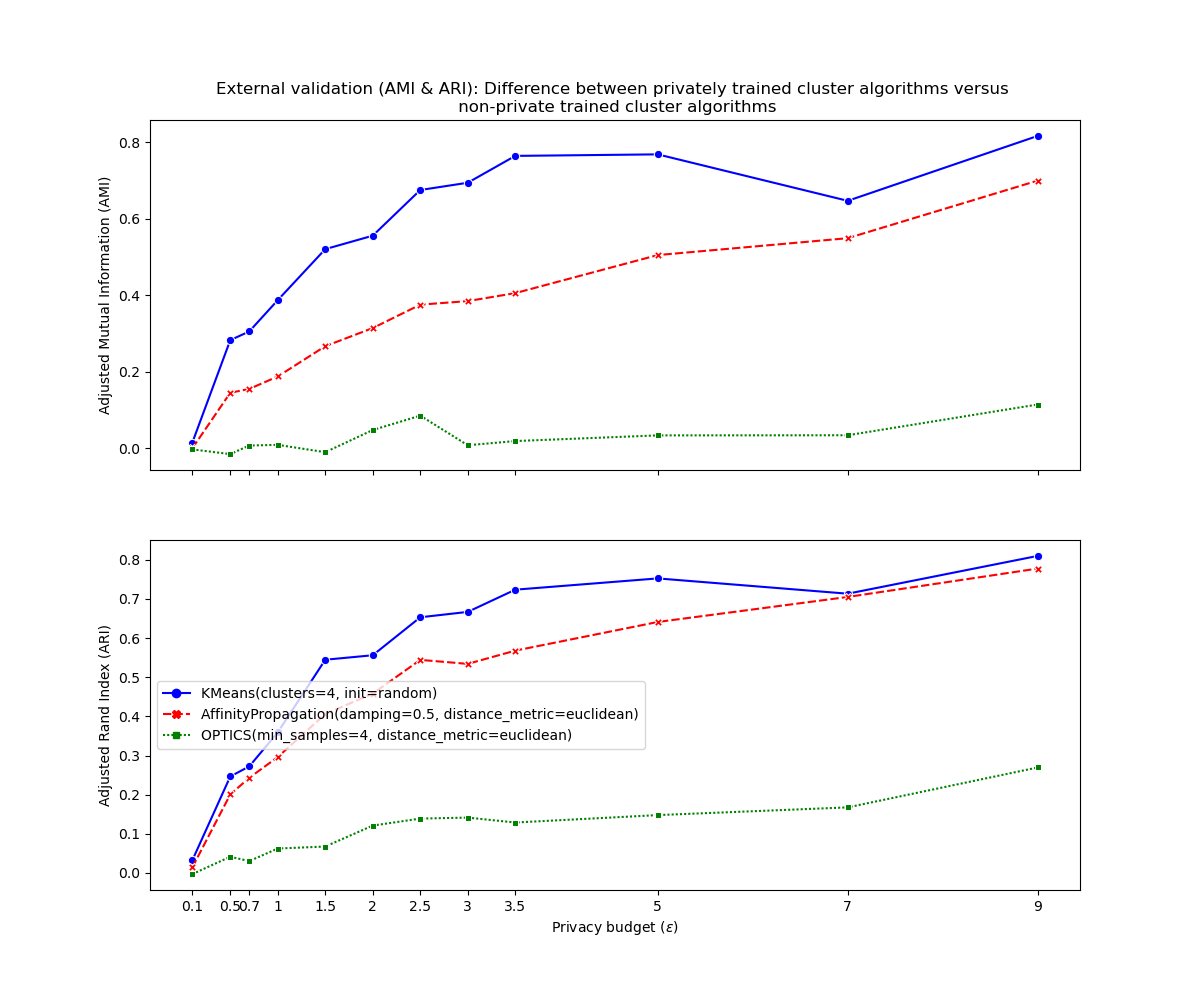
\includegraphics[width=1\textwidth]{Results/2d-laplace-optimal-truncated/seeds-dataset/ami-and-ari.png}
        \caption{External validation (ARI/ AMI) for the 2-dimensional data seeds-dataset for laplace with optimal truncation}
        \label{fig:external-validation-seeds-dataset_comparison_2d-laplace}
    \end{minipage}
    \begin{minipage}[c]{0.49\textwidth}
        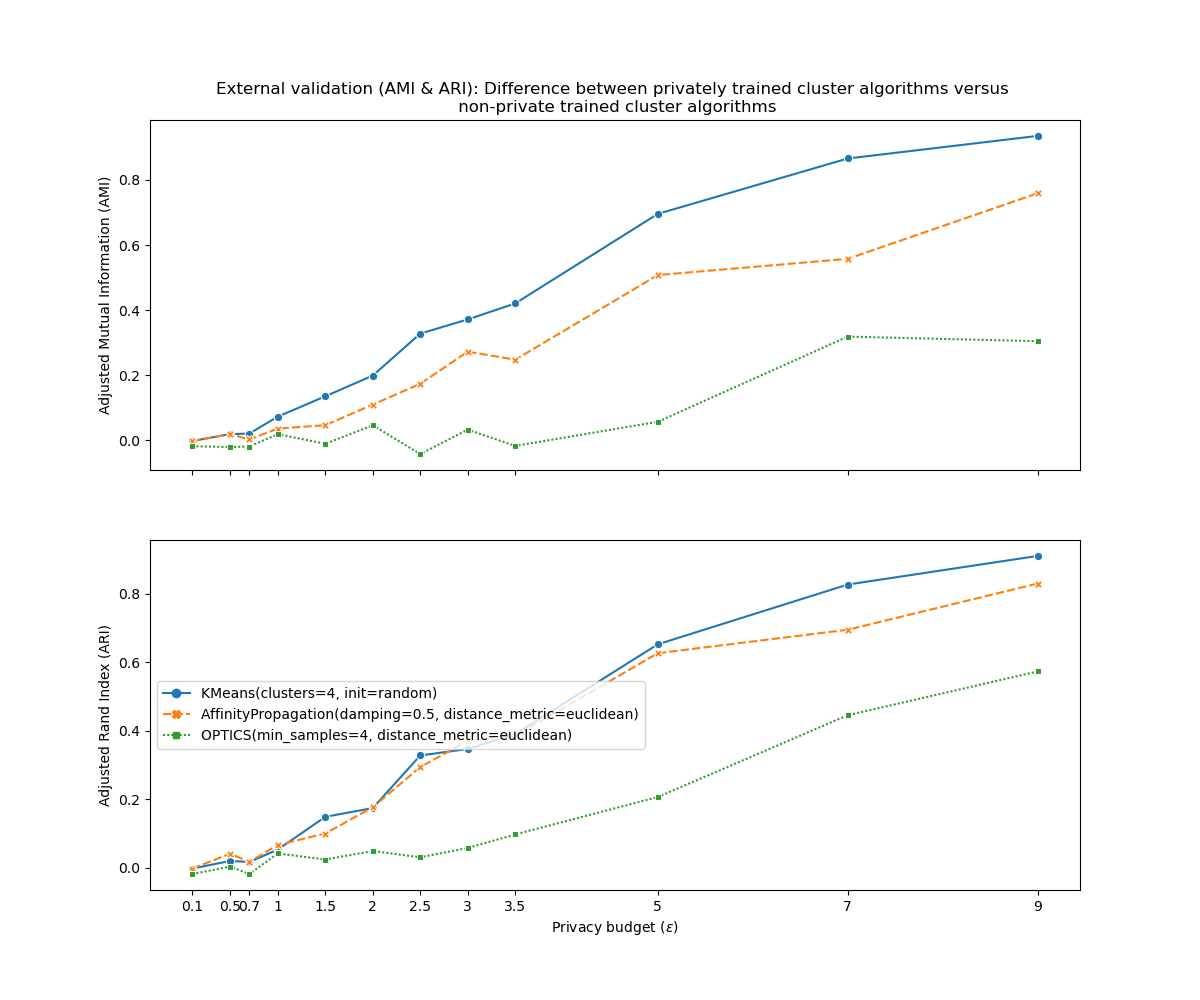
\includegraphics[width=1\textwidth]{Results/2d-piecewise/seeds-dataset/ami-and-ari.png}
        \caption{External validation (ARI/ AMI) for the 2-dimensional data seeds-dataset for piecewise mechanism}
        \label{fig:external-validation-seeds-dataset_comparison_2d-piecewise}
    \end{minipage}

\end{figure}
\begin{figure}[!htbp]
    \caption{External validation piecewise \& laplace-optimal-truncated mechanisms for the 2-dimensional data heart-dataset}
    \centering
    \begin{minipage}[c]{0.49\textwidth}
        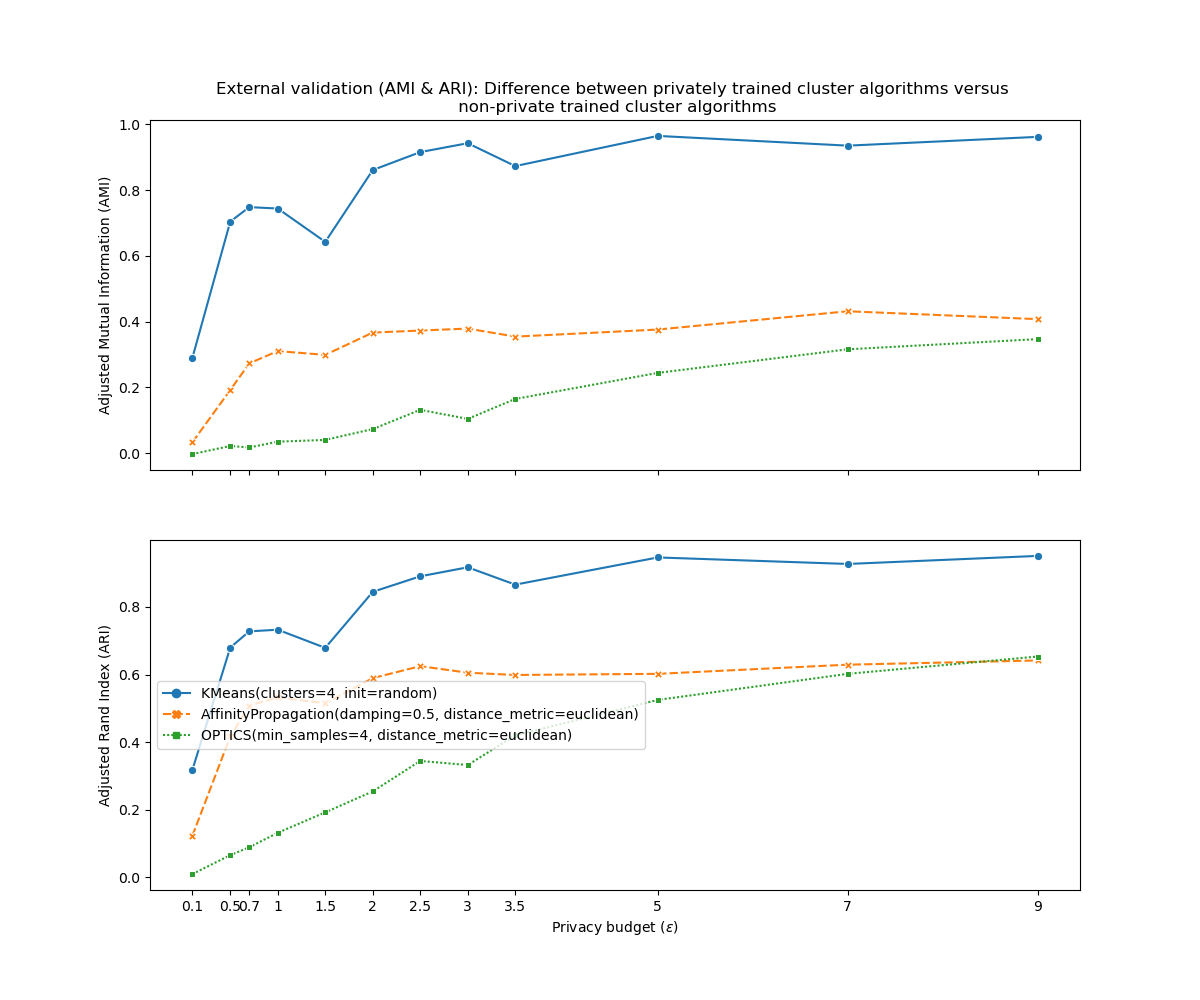
\includegraphics[width=1\textwidth]{Results/2d-laplace-optimal-truncated/heart-dataset/ami-and-ari.png}
        \caption{External validation (ARI/ AMI) for the 2-dimensional data heart-dataset for laplace with optimal truncation}
        \label{fig:external-validation-heart-dataset_comparison_2d-laplace}
    \end{minipage}
    \begin{minipage}[c]{0.49\textwidth}
        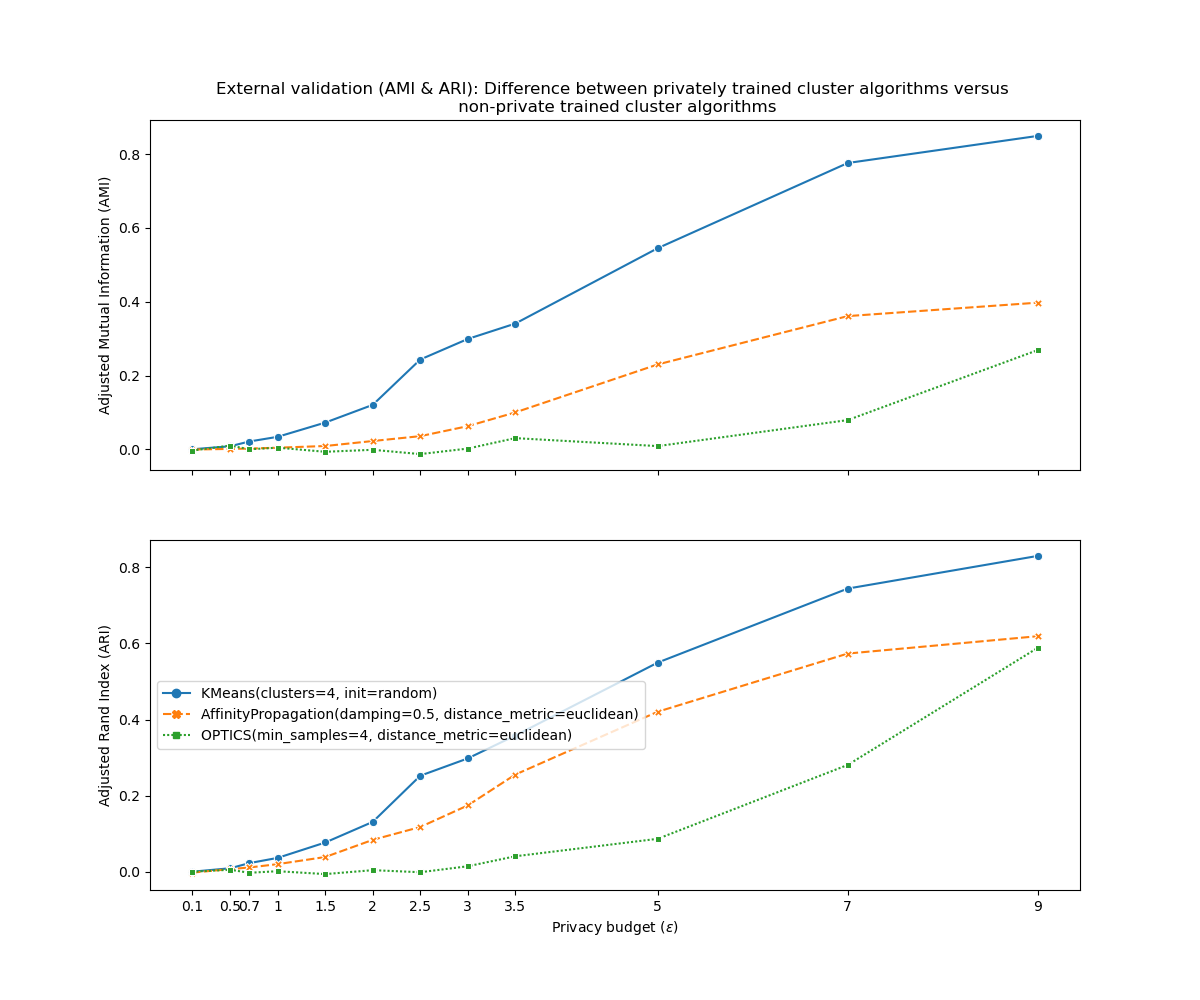
\includegraphics[width=1\textwidth]{Results/2d-piecewise/heart-dataset/ami-and-ari.png}
        \caption{External validation (ARI/ AMI) for the 2-dimensional data heart-dataset for piecewise mechanism}
        \label{fig:external-validation-heart-dataset_comparison_2d-piecewise}
    \end{minipage}
\end{figure}
\subsection{3-dimensional data}
\begin{figure}[H]
    \caption{External validation piecewise \& laplace-optimal-truncated mechanisms for the 3-dimensional data seeds-dataset}
    \centering
    \begin{minipage}[c]{0.49\textwidth}
        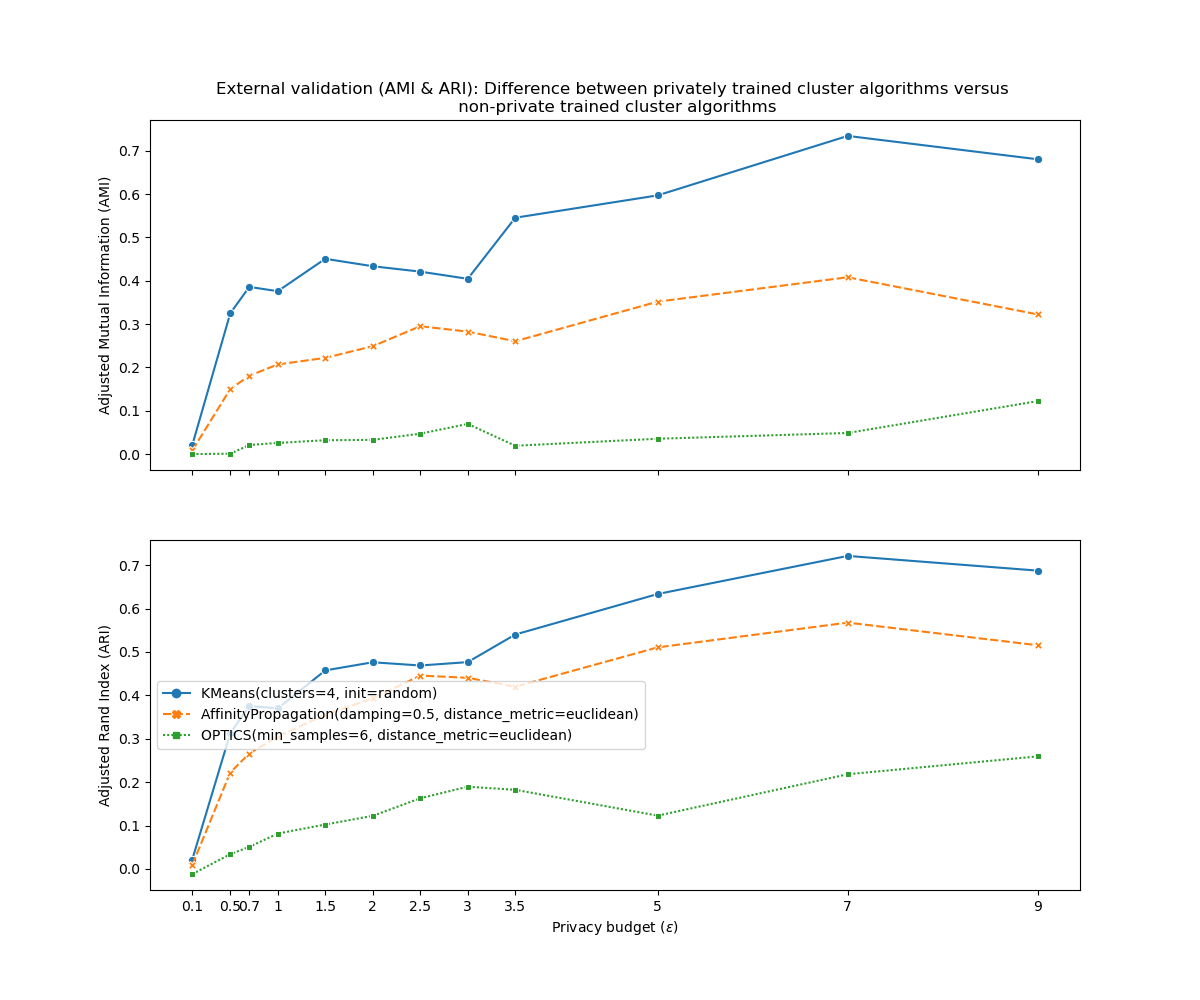
\includegraphics[width=1\textwidth]{Results/3d-laplace-optimal-truncated/seeds-dataset/ami-and-ari.png}
        \caption{External validation (ARI/ AMI) for the 3-dimensional data seeds-dataset for laplace with optimal truncation}
        \label{fig:external-validation-seeds-dataset_comparison_3d-laplace}
    \end{minipage}
    \begin{minipage}[c]{0.49\textwidth}
        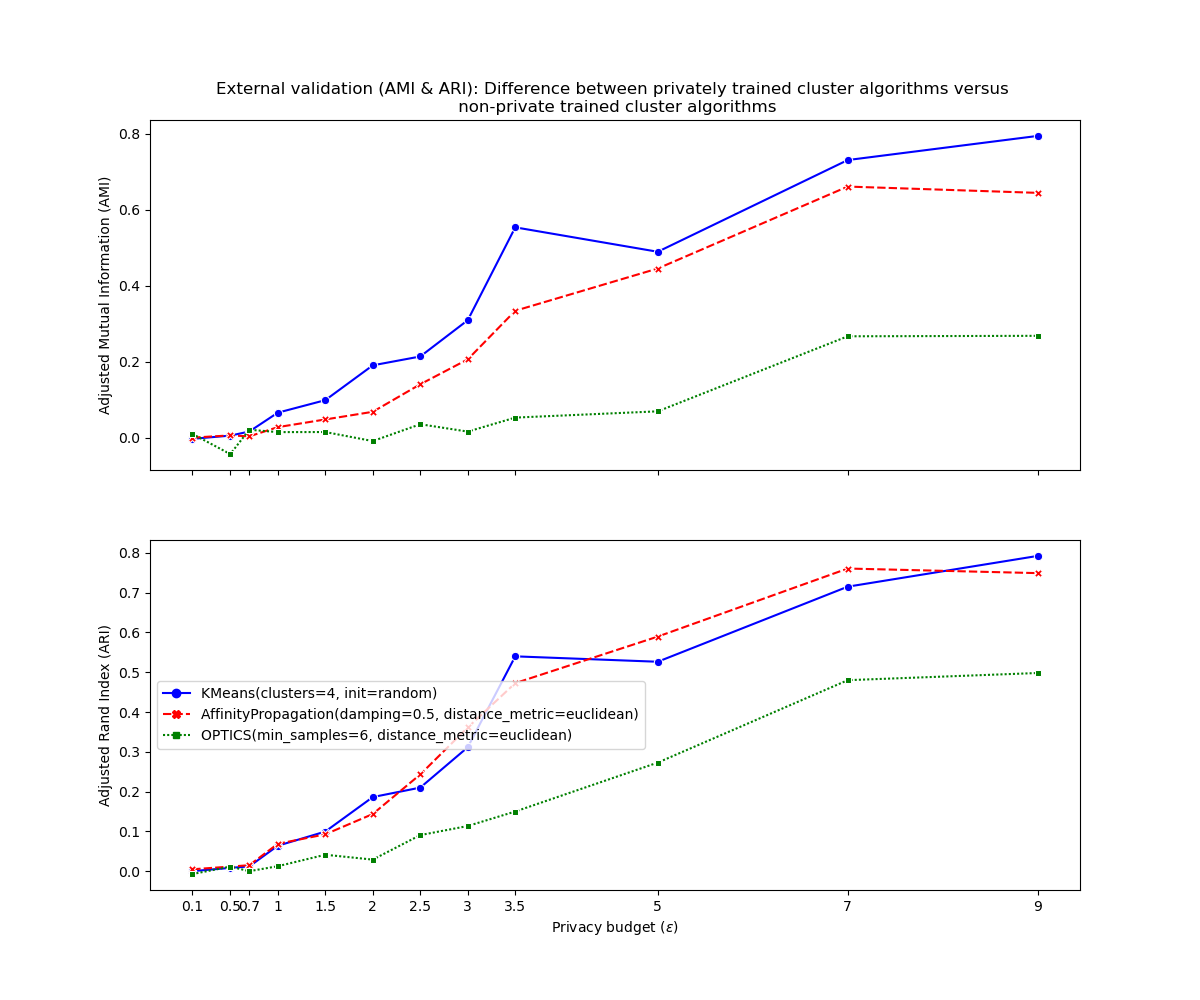
\includegraphics[width=1\textwidth]{Results/3d-piecewise/seeds-dataset/ami-and-ari.png}
        \caption{External validation (ARI/ AMI) for the 3-dimensional data seeds-dataset for piecewise mechanism}
        \label{fig:external-validation-seeds-dataset_comparison_3d-piecewise}
    \end{minipage}

\end{figure}
\begin{figure}[H]
    \caption{External validation piecewise \& laplace-optimal-truncated mechanisms for the 3-dimensional data heart-dataset}
    \centering
    \begin{minipage}[c]{0.49\textwidth}
        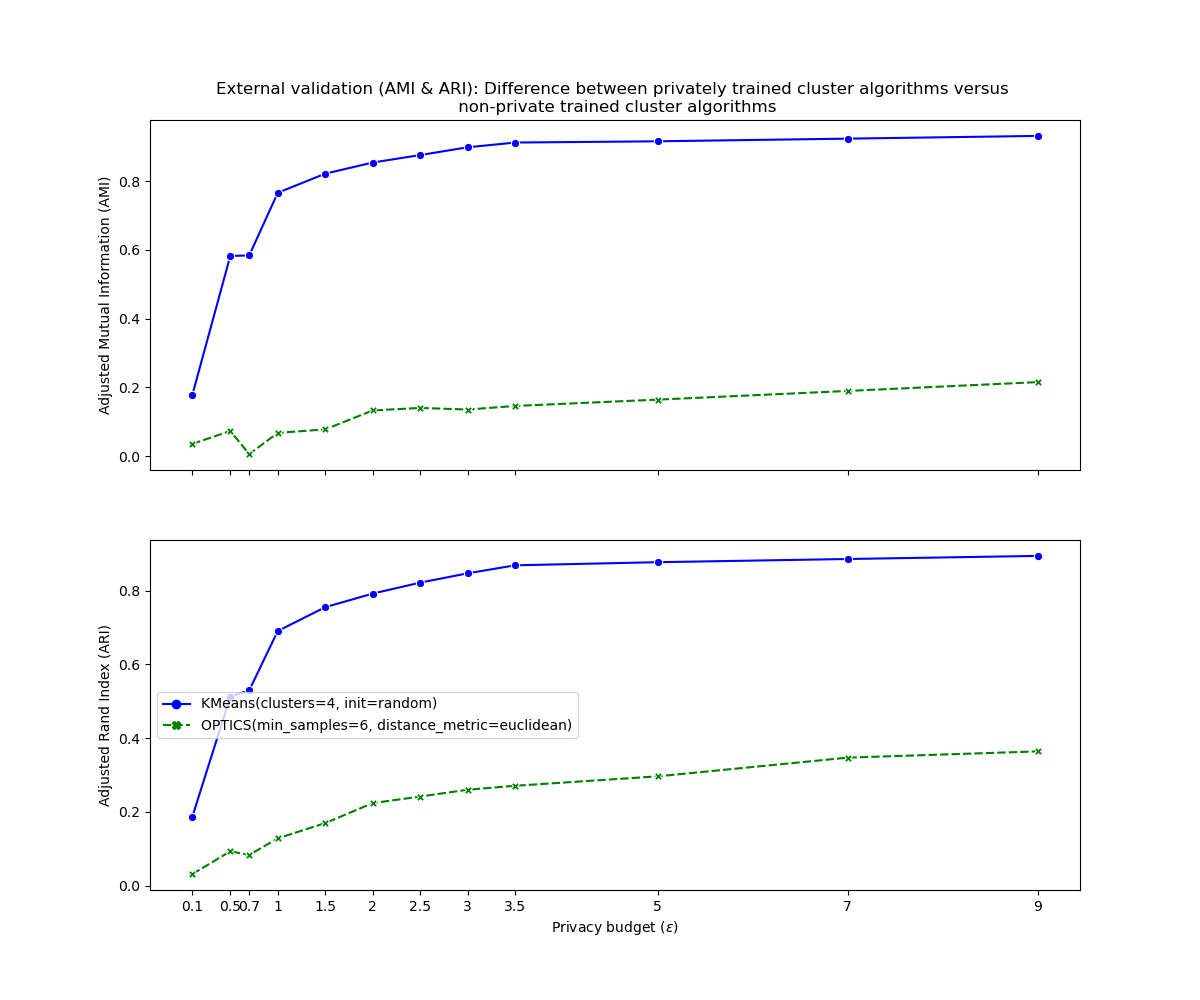
\includegraphics[width=1\textwidth]{Results/3d-laplace-optimal-truncated/heart-dataset/ami-and-ari.png}
        \caption{External validation (ARI/ AMI) for the 3-dimensional data heart-dataset for laplace with optimal truncation}
        \label{fig:external-validation-heart-dataset_comparison_3d-laplace}
    \end{minipage}
    \begin{minipage}[c]{0.49\textwidth}
        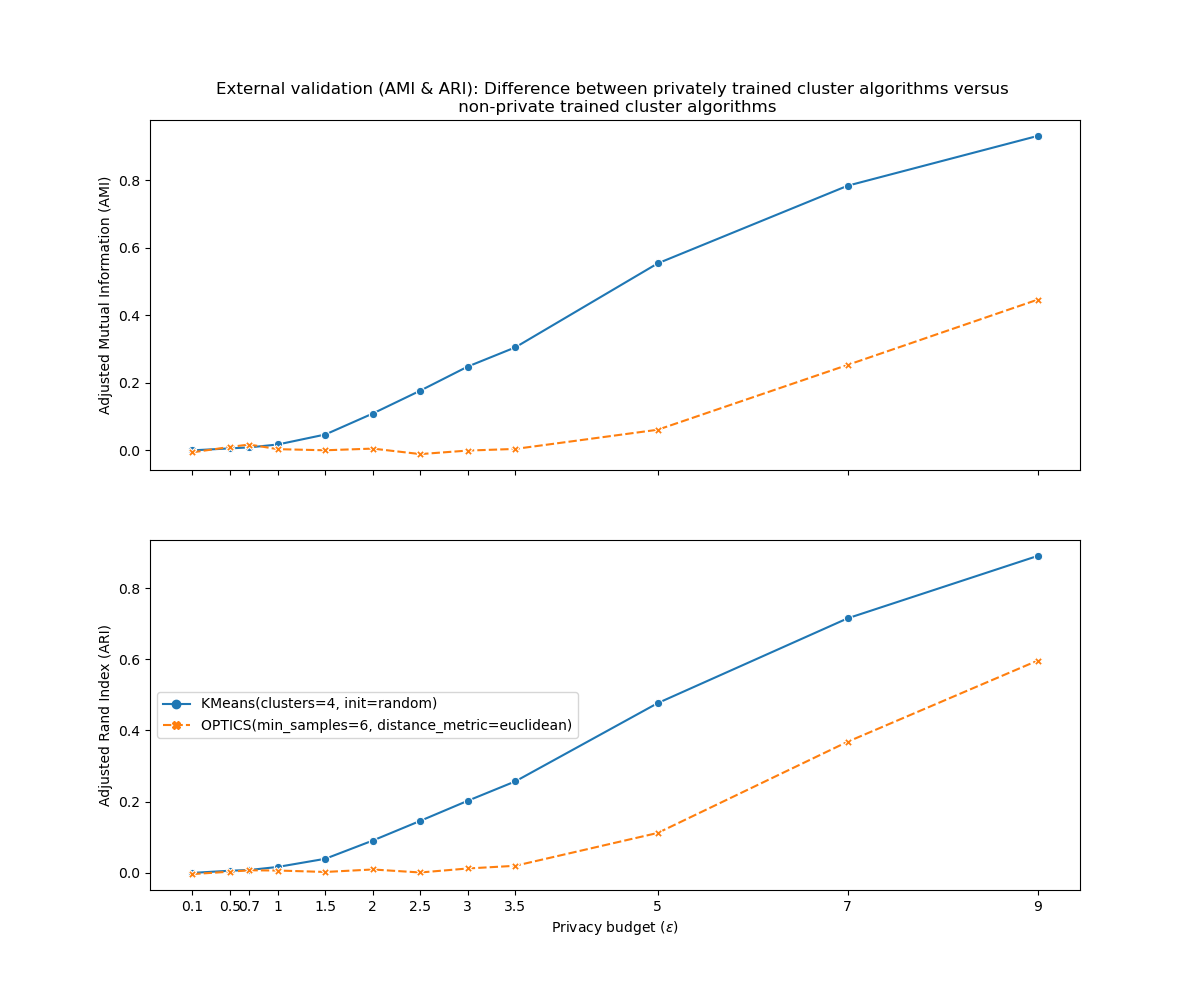
\includegraphics[width=1\textwidth]{Results/3d-piecewise/heart-dataset/ami-and-ari.png}
        \caption{External validation (ARI/ AMI) for the 3-dimensional data heart-dataset for piecewise mechanism}
        \label{fig:external-validation-heart-dataset_comparison_3d-piecewise}
    \end{minipage}
\end{figure}
\subsection{n-dimensional data}
\begin{figure}[H]
    \caption{External validation piecewise \& laplace-optimal-truncated mechanisms for the n-dimensional data seeds-dataset}
    \centering
    \begin{minipage}[c]{0.49\textwidth}
        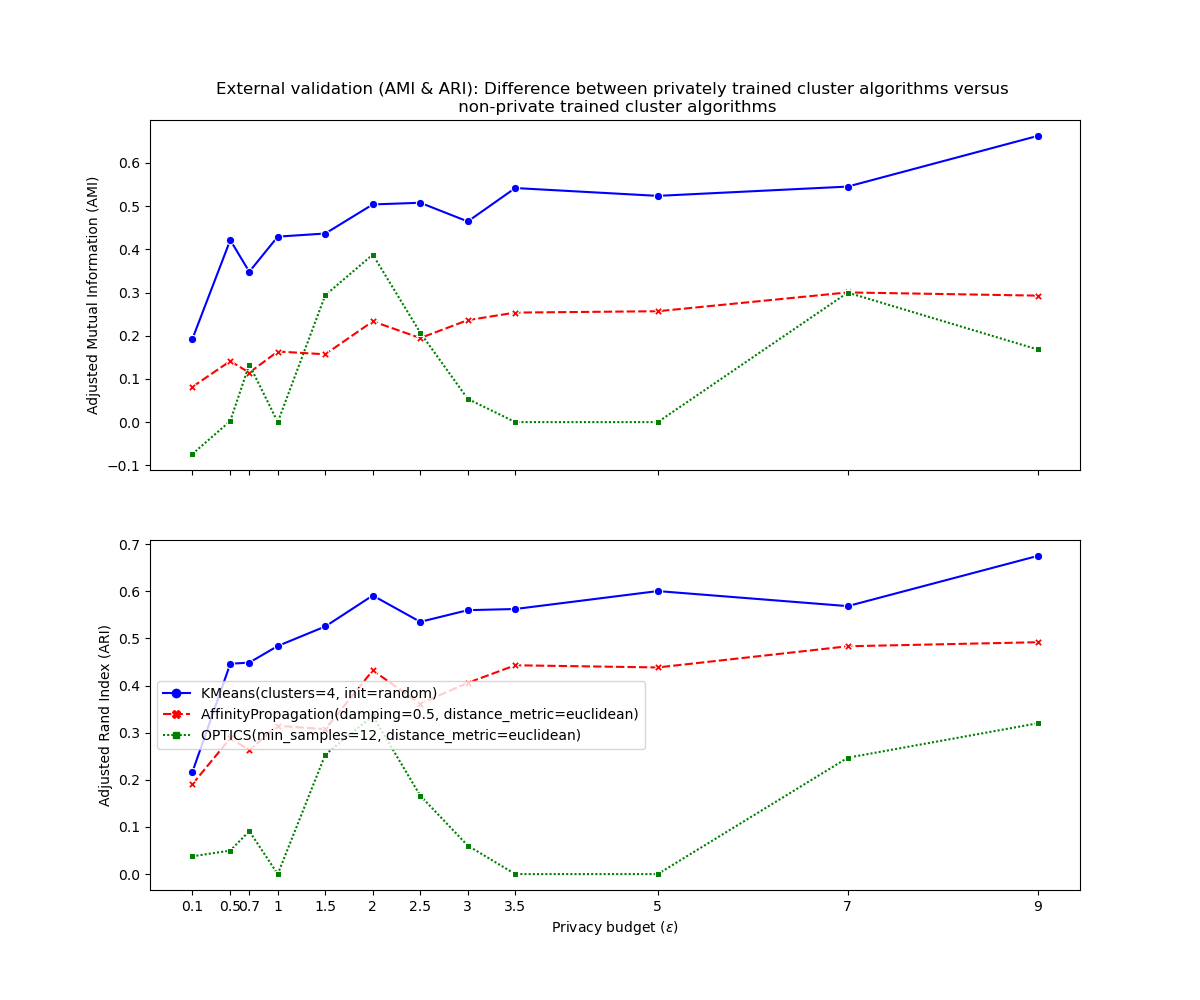
\includegraphics[width=1\textwidth]{Results/nd-laplace-optimal-truncated/seeds-dataset/ami-and-ari.png}
        \caption{External validation (ARI/ AMI) for the n-dimensional data seeds-dataset for laplace with optimal truncation}
        \label{fig:external-validation-seeds-dataset_comparison_nd-laplace}
    \end{minipage}
    \begin{minipage}[c]{0.49\textwidth}
        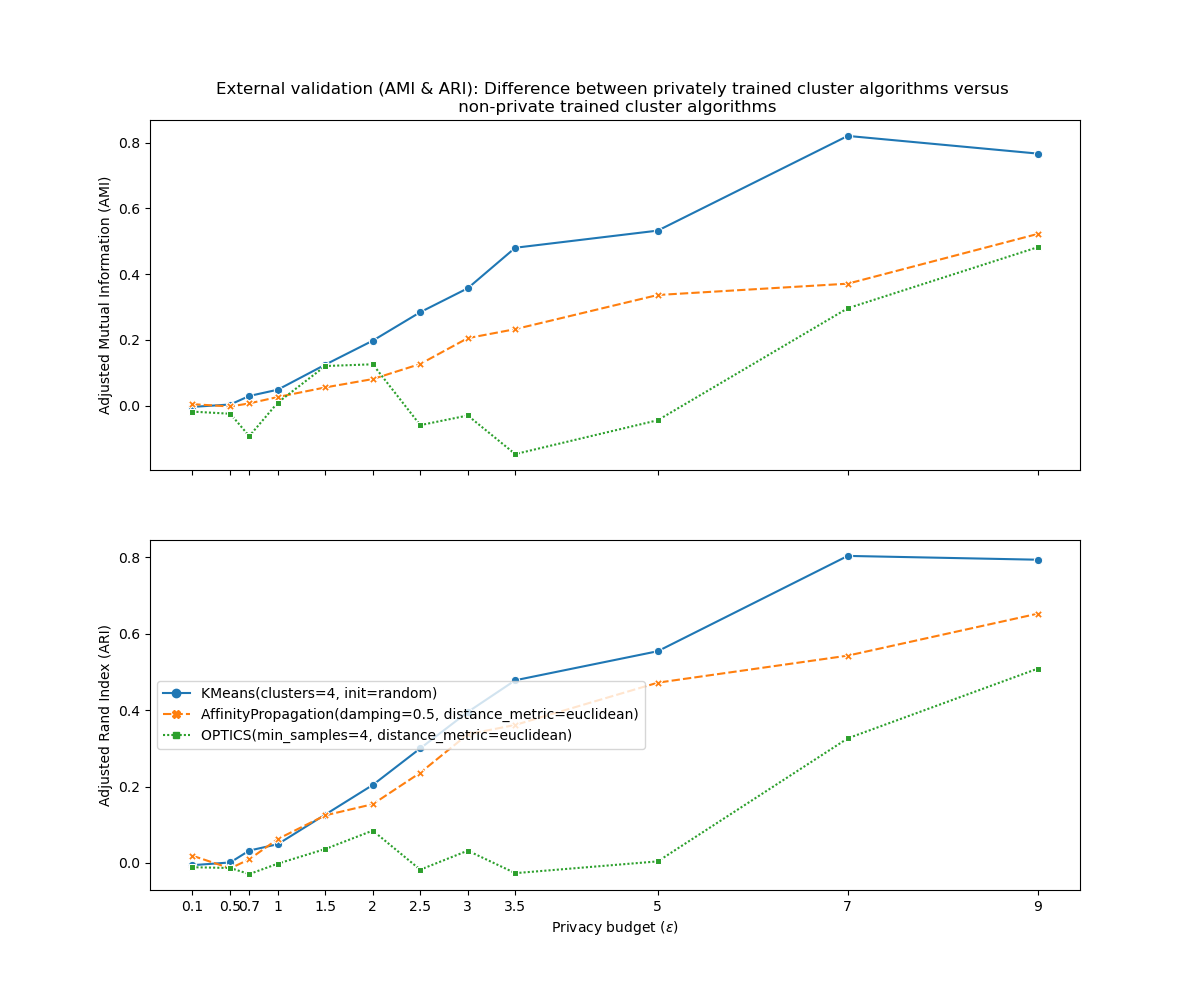
\includegraphics[width=1\textwidth]{Results/nd-piecewise/seeds-dataset/ami-and-ari.png}
        \caption{External validation (ARI/ AMI) for the n-dimensional data seeds-dataset for piecewise mechanism}
        \label{fig:external-validation-seeds-dataset_comparison_nd-piecewise}
    \end{minipage}
\end{figure}
\begin{figure}[H]
    \caption{External validation piecewise \& laplace-optimal-truncated mechanisms for the n-dimensional data heart-dataset}
    \centering
    \begin{minipage}[c]{0.49\textwidth}
        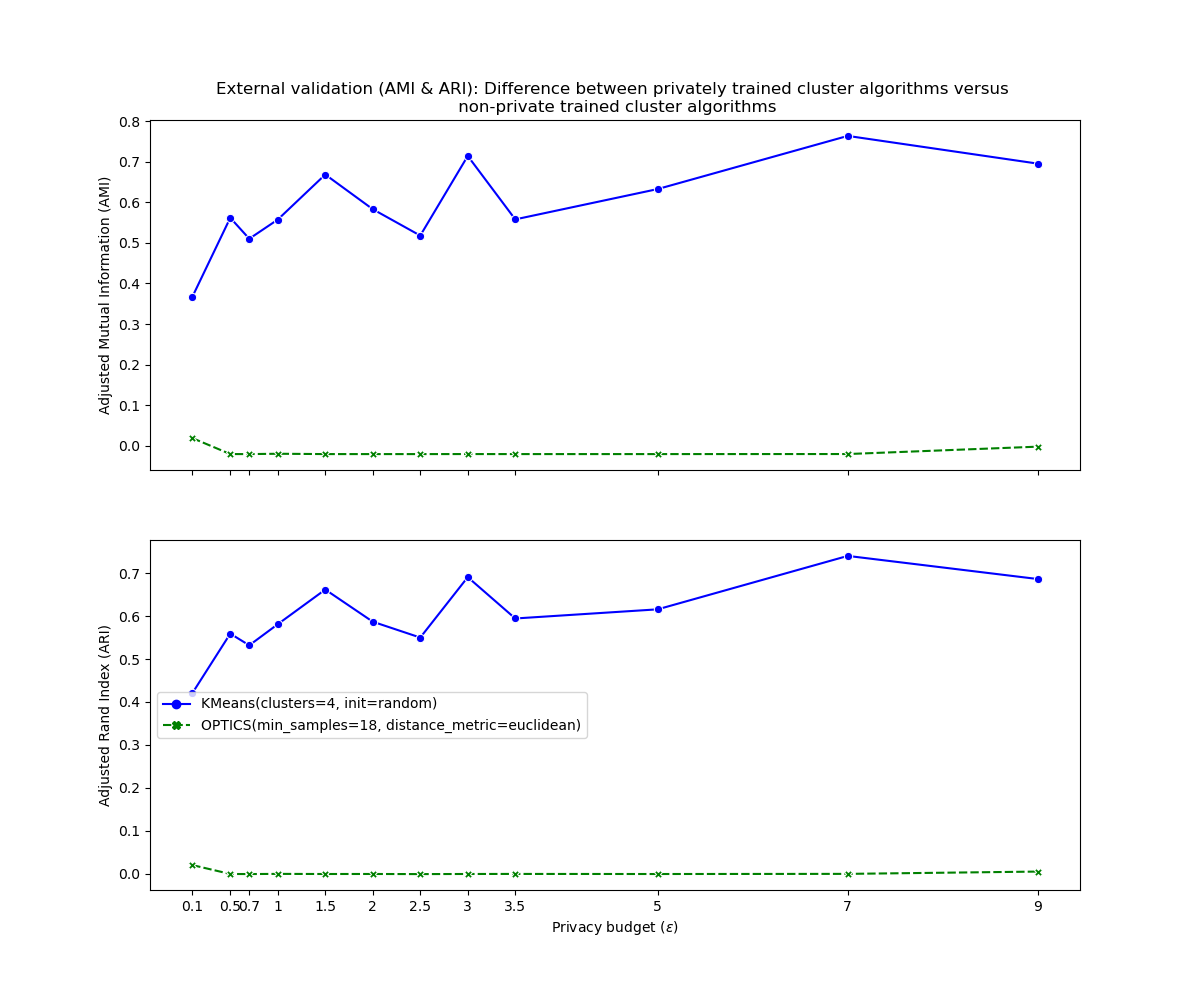
\includegraphics[width=1\textwidth]{Results/nd-laplace-optimal-truncated/heart-dataset/ami-and-ari.png}
        \caption{External validation (ARI/ AMI) for the n-dimensional data heart-dataset for laplace with optimal truncation}
        \label{fig:external-validation-heart-dataset_comparison_nd-laplace}
    \end{minipage}
    \begin{minipage}[c]{0.49\textwidth}
        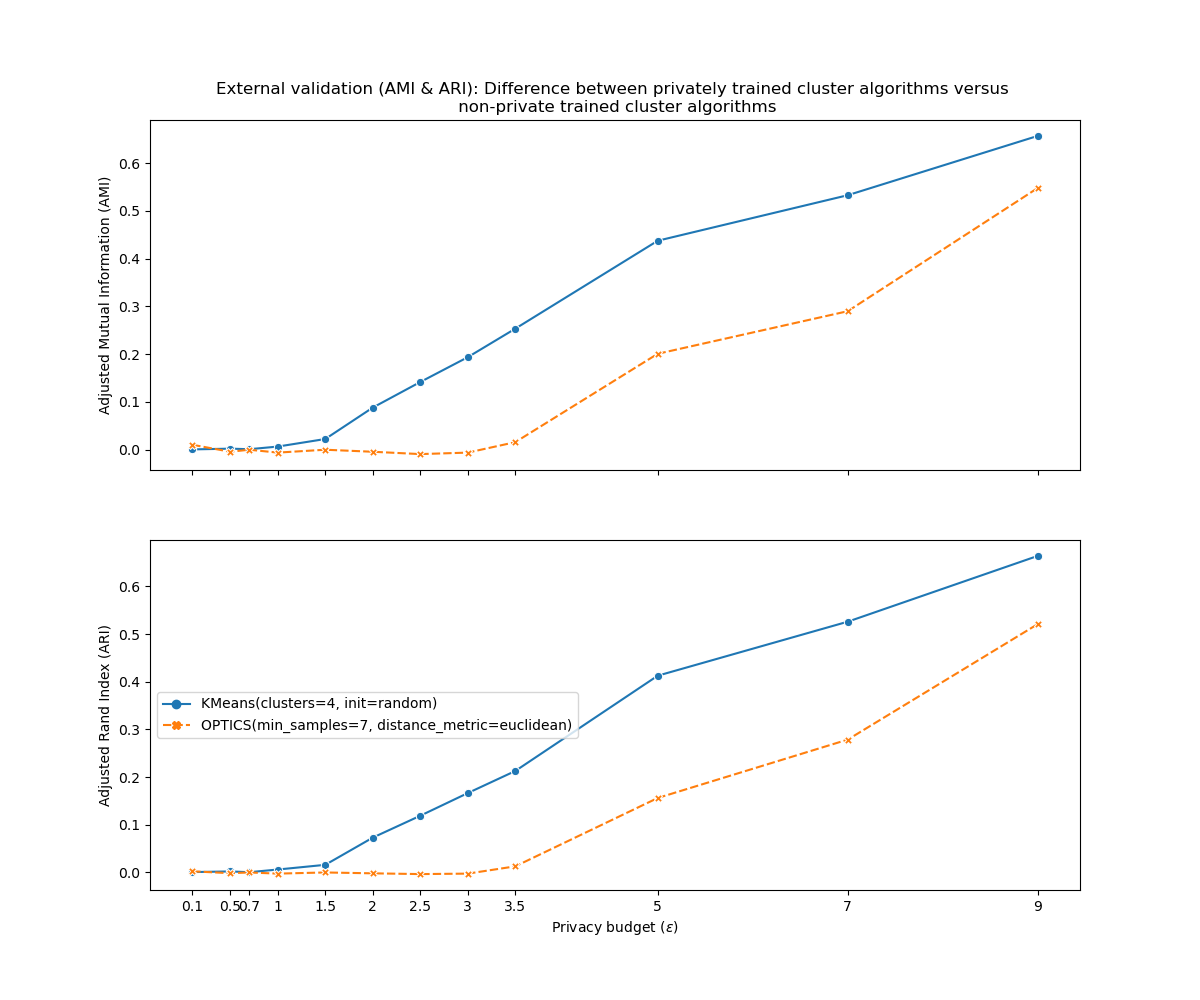
\includegraphics[width=1\textwidth]{Results/nd-piecewise/heart-dataset/ami-and-ari.png}
        \caption{External validation (ARI/ AMI) for the n-dimensional data heart-dataset for piecewise mechanism}
        \label{fig:external-validation-heart-dataset_comparison_nd-piecewise}
    \end{minipage}
\end{figure}
\newpage
\section{Mechanism utility}
In the images below, the different types of Laplace mechanisms and piecewise are compared using a barplot.
Since both ARI and AMI provide the same information, we have chosen to show only the Adjusted Mutual Information (AMI) to avoid redundant information. For the same reason, only the K-Means algorithm was used to calculate the AMI.
The x-axis displays the privacy budget, and the y-axis shows the corresponding AMI.
\todo[inline]{Add links to scilliouette plots and other plots}

\subsection{2-dimensional data}
\begin{figure}[H]
    \centering
    \begin{minipage}[c]{0.8\textwidth}
        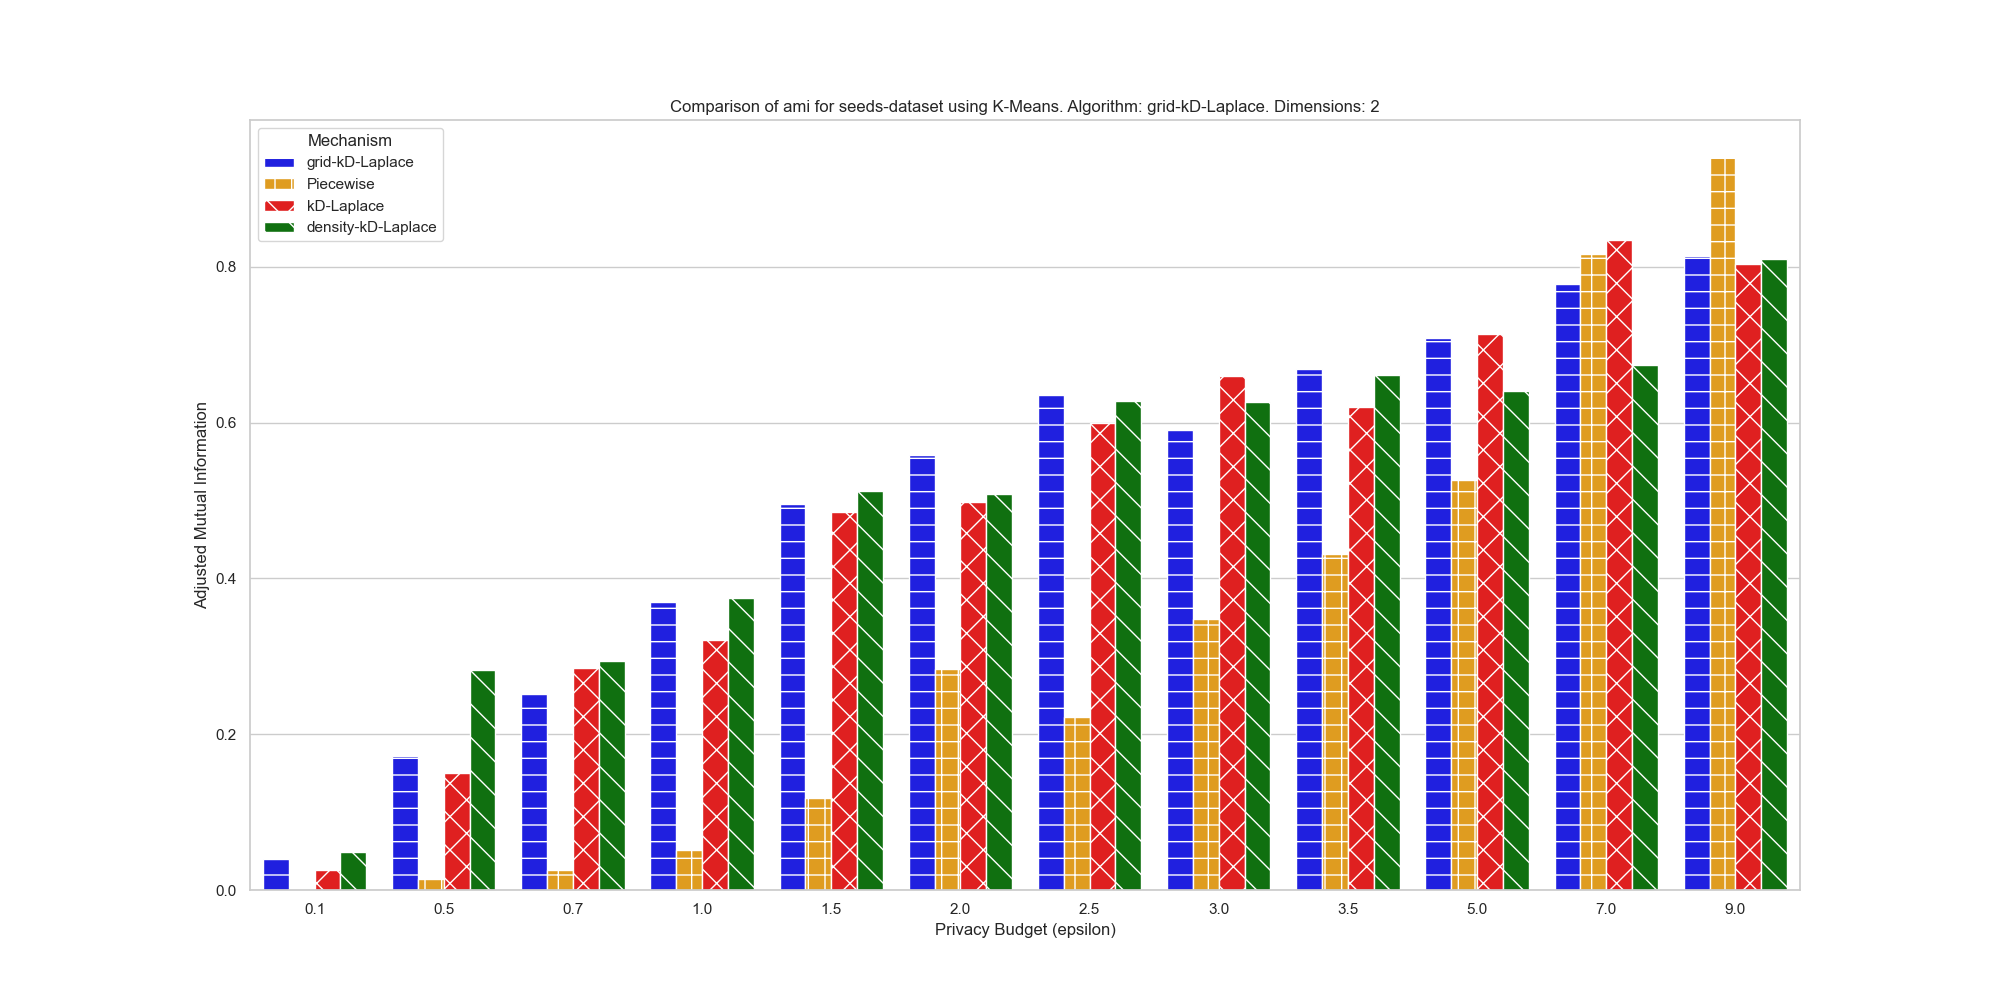
\includegraphics[width=1\textwidth]{Results/RQ1/seeds-dataset/ami_seeds-dataset_comparison.png}
        \caption{Adjusted Mutual Information comparison for the seeds-dataset}
        \label{fig:ami_seeds-dataset_comparison_2d}
    \end{minipage}
    \begin{minipage}[c]{0.8\textwidth}
        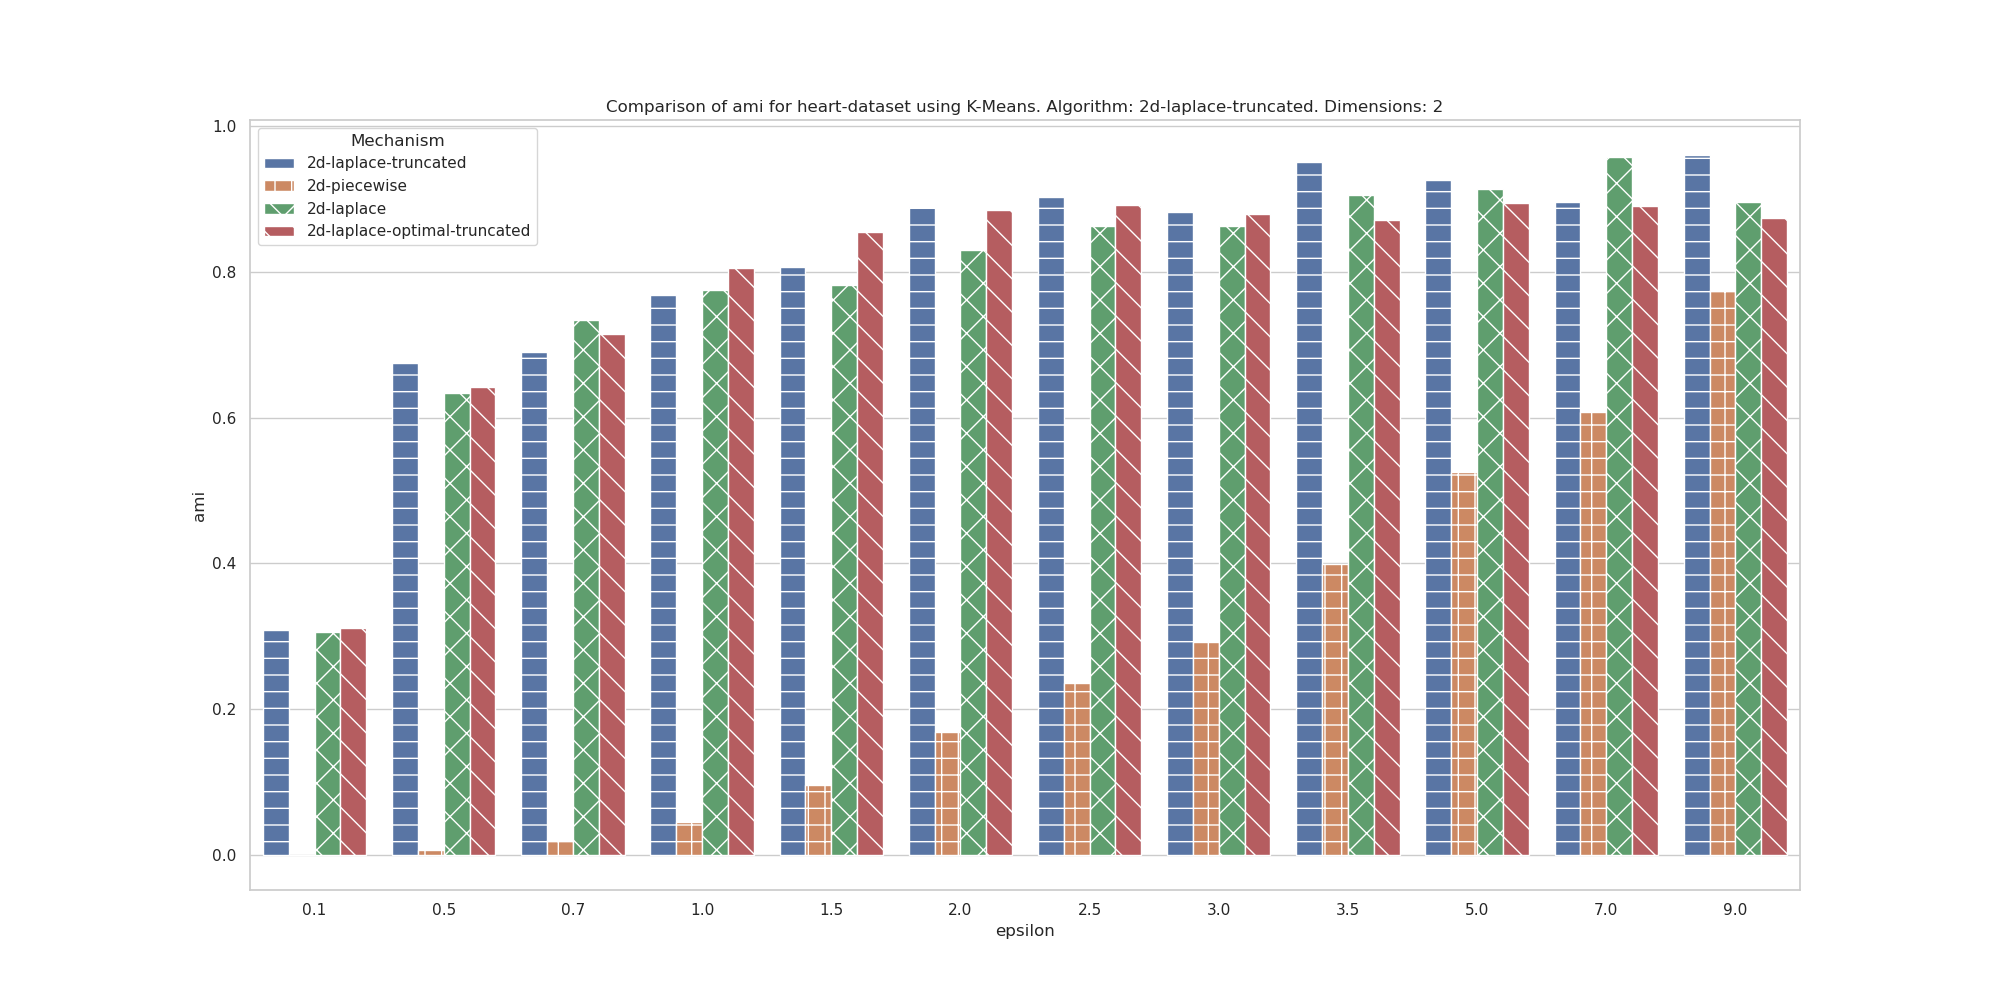
\includegraphics[width=1\textwidth]{Results/RQ1/heart-dataset/ami_heart-dataset_comparison.png}
        \caption{Adjusted Mutual Information comparison for the heart-dataset}
        \label{fig:ami_heart-dataset_comparison_2d}
    \end{minipage}

\end{figure}

\newpage
\subsection{3-dimensional data}
\begin{figure}[H]
    \centering
    \begin{minipage}[c]{0.8\textwidth}
        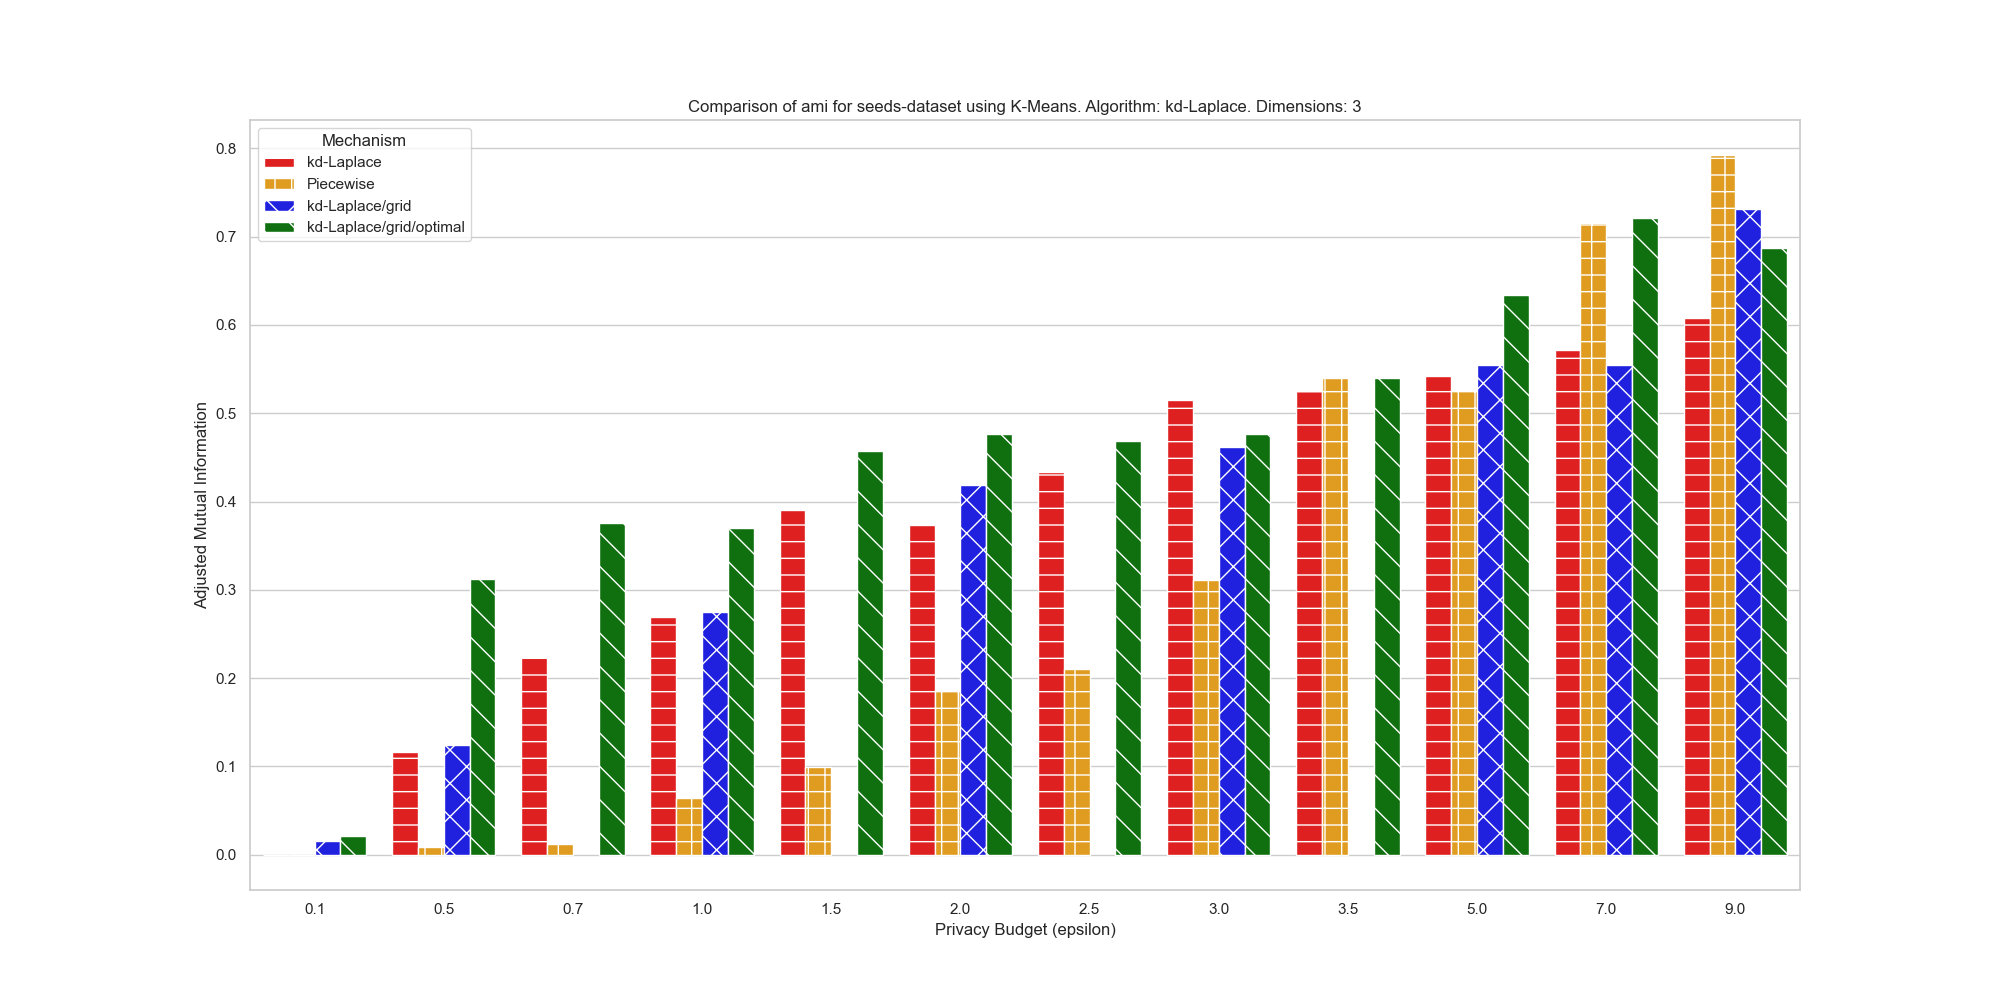
\includegraphics[width=1\textwidth]{Results/RQ2/seeds-dataset/ami_seeds-dataset_comparison.png}
        \caption{Adjusted Mutual Information comparison for the 3-dimensional seeds-dataset}
        \label{fig:ami_seeds-dataset_comparison_3d}
    \end{minipage}
    \begin{minipage}[c]{0.8\textwidth}
        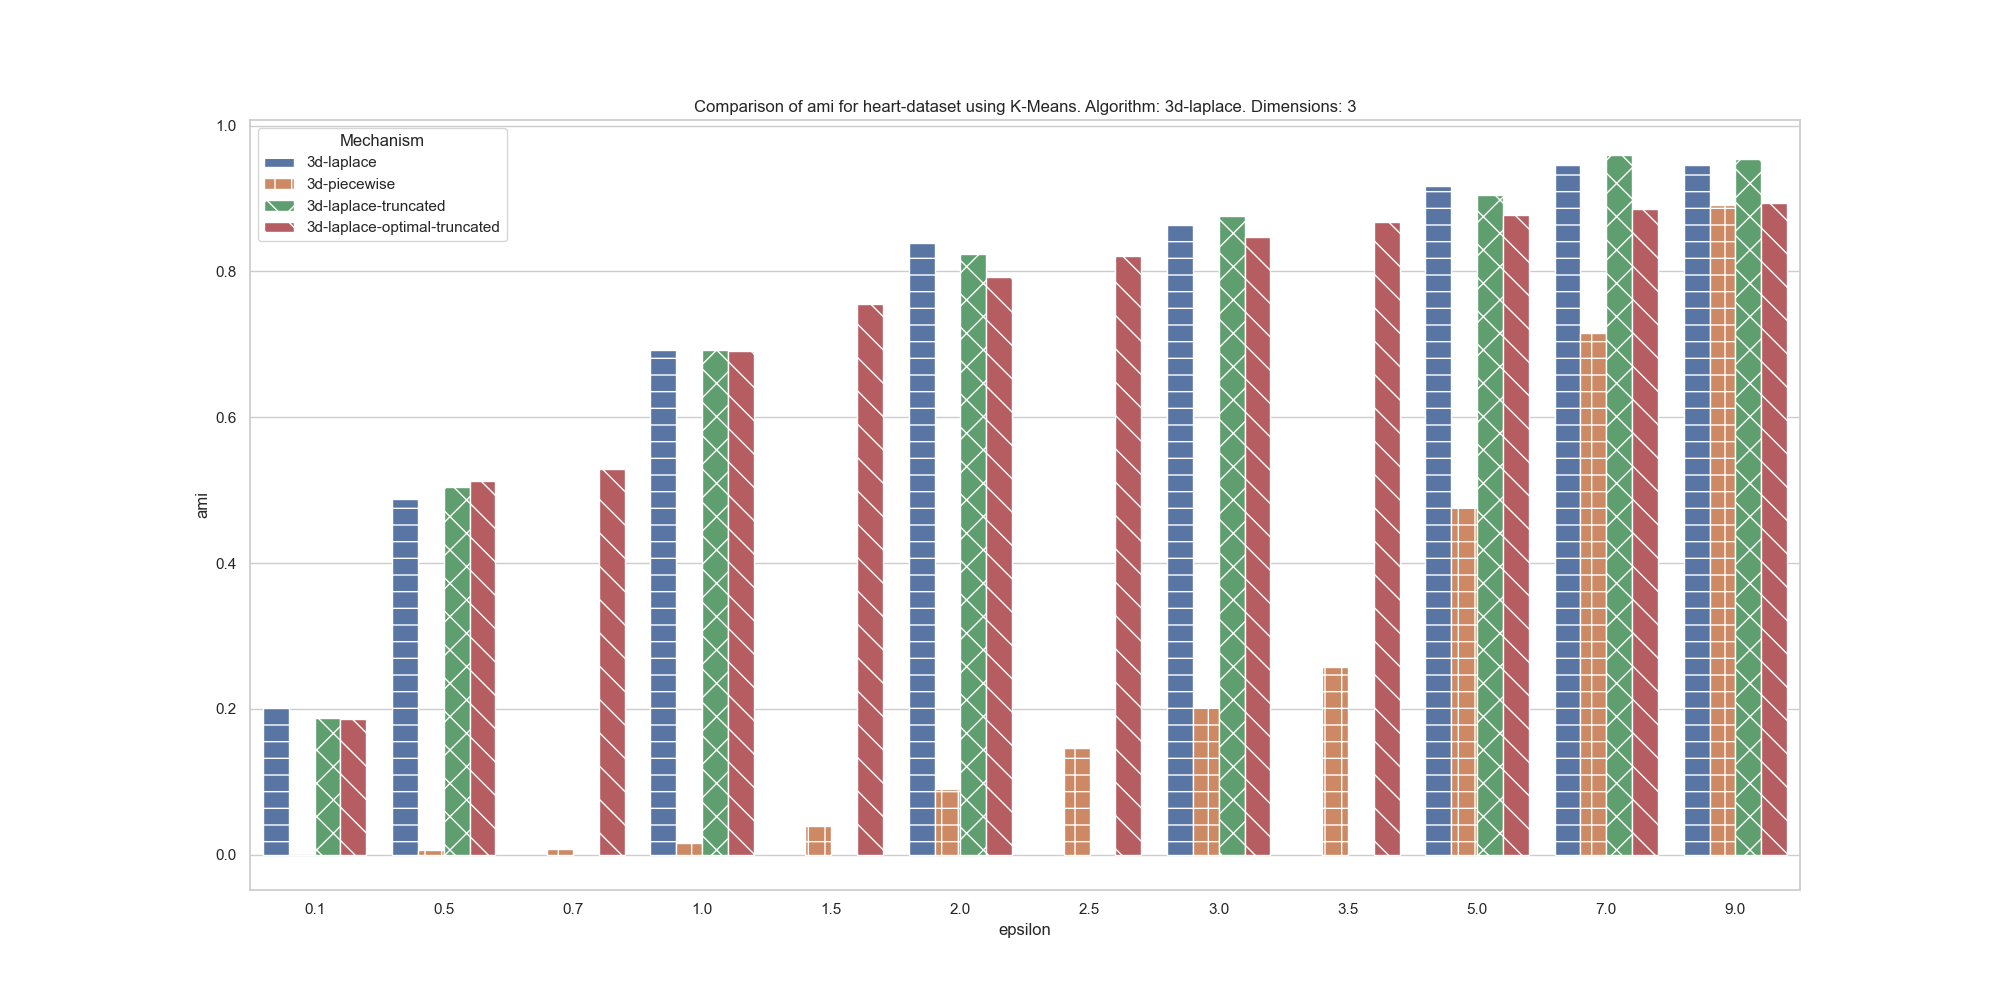
\includegraphics[width=1\textwidth]{Results/RQ2/heart-dataset/ami_heart-dataset_comparison.png}
        \caption{Adjusted Mutual Information comparison for the 3-dimensional heart-dataset}
        \label{fig:ami_heart-dataset_comparison_3d}
    \end{minipage}

\end{figure}
\newpage
\subsection{n-dimensional data}
\begin{figure}[H]
    \centering
    \begin{minipage}[c]{0.8\textwidth}
        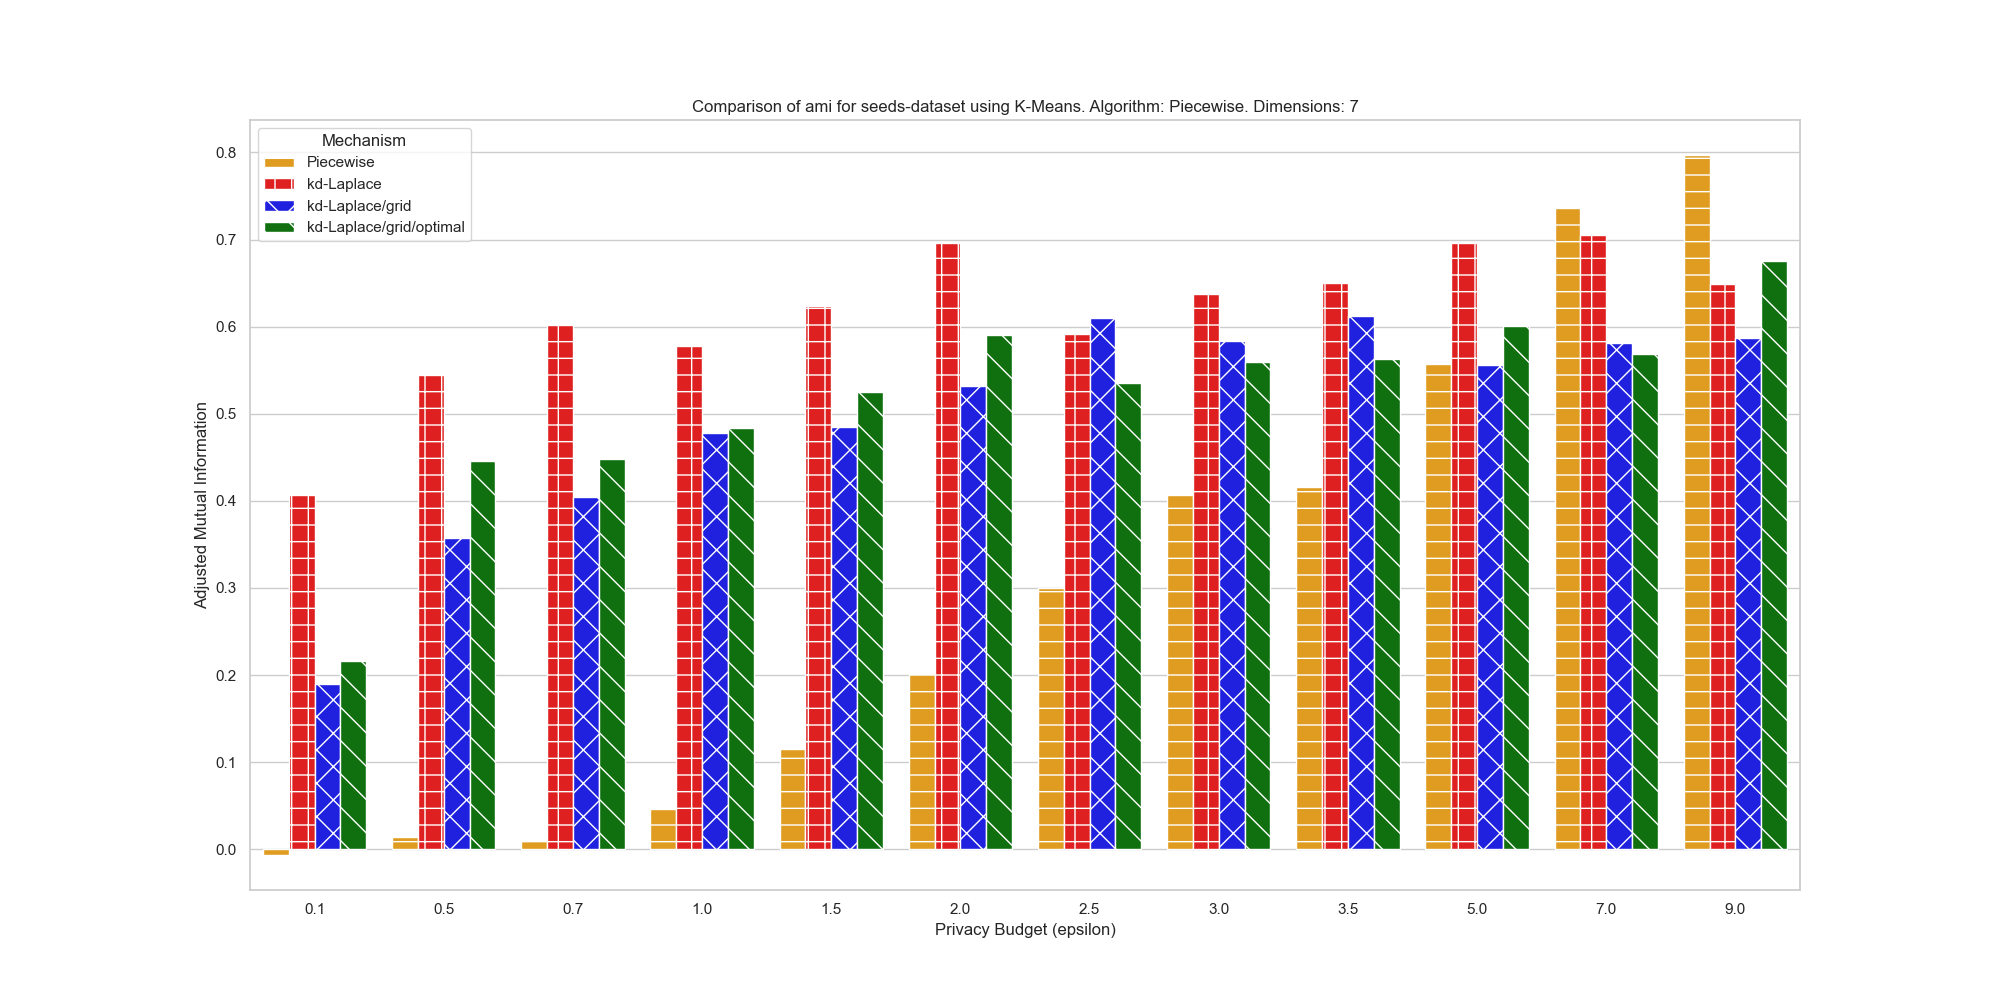
\includegraphics[width=1\textwidth]{Results/RQ2-nd/seeds-dataset/ami_seeds-dataset_comparison.png}
        \caption{Adjusted Mutual Information comparison for all numerical features for the seeds-dataset}
        \label{fig:ami_seeds-dataset_comparison_nd}
    \end{minipage}
    \begin{minipage}[c]{0.8\textwidth}
        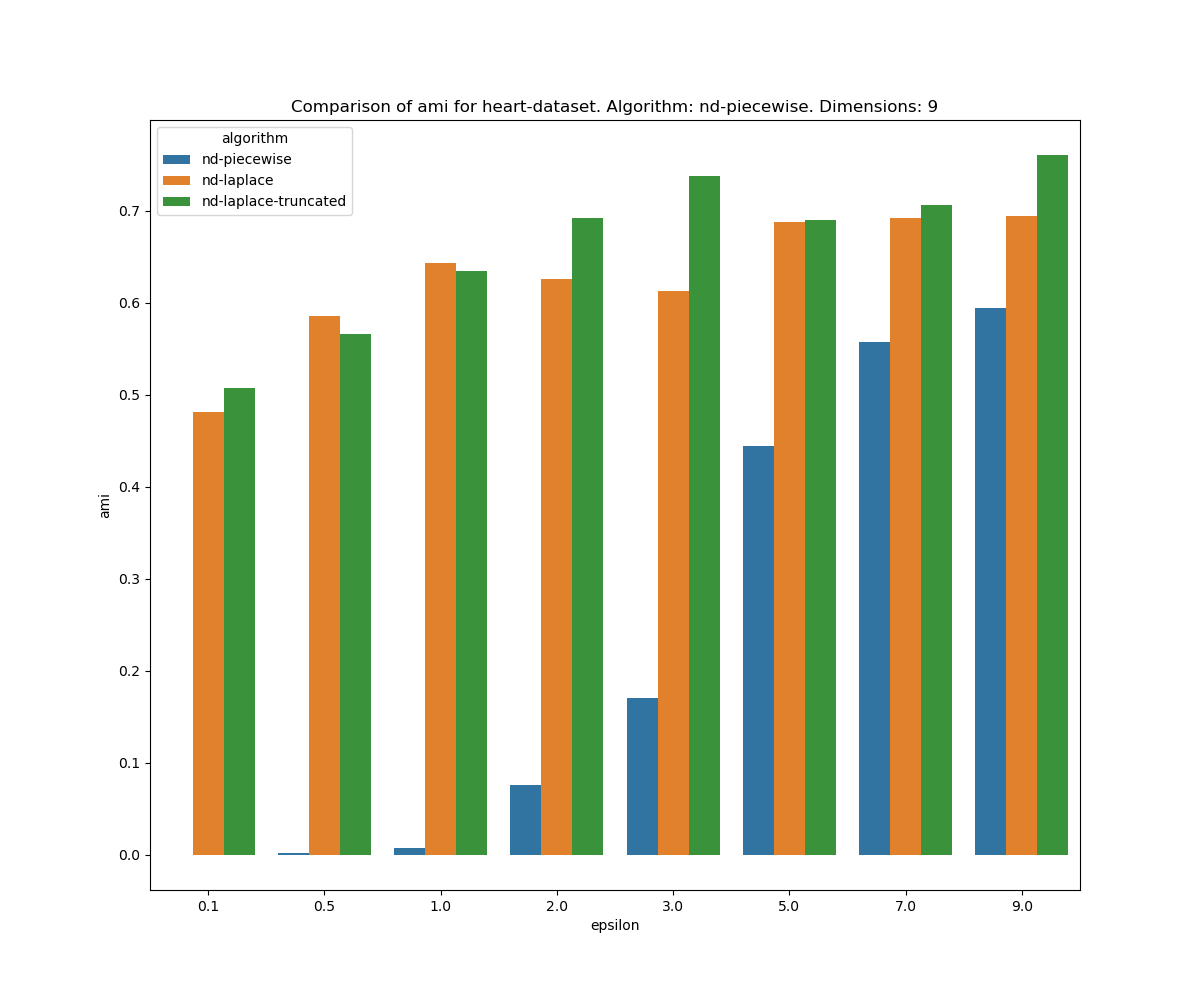
\includegraphics[width=1\textwidth]{Results/RQ2-nd/heart-dataset/ami_heart-dataset_comparison.png}
        \caption{Adjusted Mutual Information comparison for all numerical features for the heart-dataset}
        \label{fig:ami_heart-dataset_comparison_nd}
    \end{minipage}

\end{figure}
\newpage
\section{Privacy}
The images below display a ROC curve plot of membership inference attacks as described in the methodology.
There are three baseline values: The red and green dashed lines represent the baseline True Positive Rate (TPR) and False Positive Rate (FPR), respectively. These baselines represent the attack without using any privacy mechanism. The "random guess" is the baseline for the ROC curve and reflects the 50\% chance that an adversary has in determining whether a data point is a member. Anything above this baseline can be considered an improvement in that chance.
The y-axis represents the TPR, and the x-axis represents the FPR. For each mechanism, a ROC curve is shown using different lines.
Finally, we provide a table with the mechanism and mean of the epsilon that is outside the specification of the TPR (TPR of the non-private dataset).
\subsection{2-dimensional data}
\begin{figure}[H]
    \centering
    \begin{minipage}[c]{0.49\textwidth}
        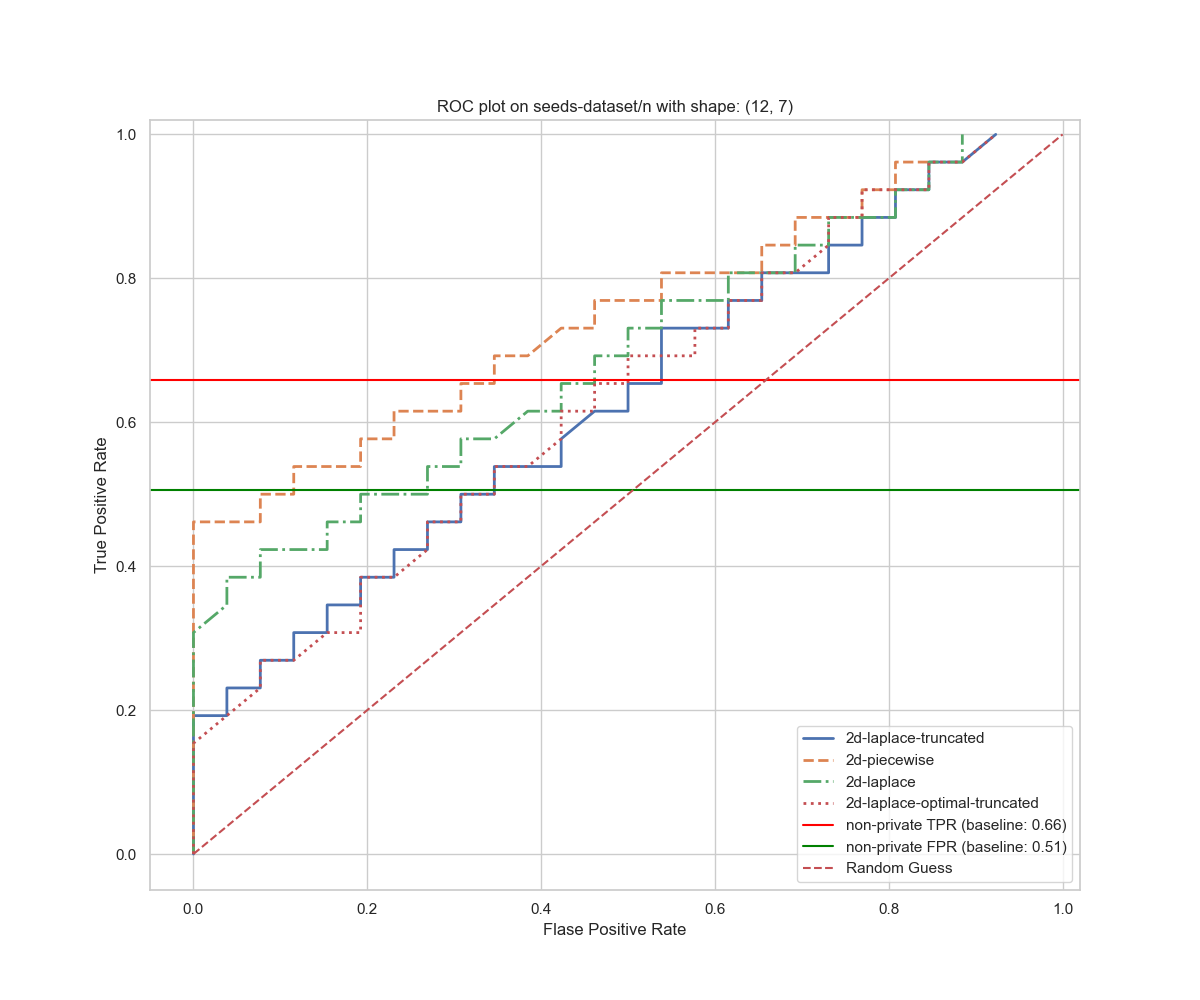
\includegraphics[width=1\textwidth]{Results/RQ1/seeds-dataset/roc_plot.png}
        \caption{ROC-curve for privacy per privacy mechanism for seeds-dataset.}
        \label{fig:privacy_seeds-dataset_comparison_2d_roc_plot}
    \end{minipage}
    \begin{minipage}[c]{0.49\textwidth}
        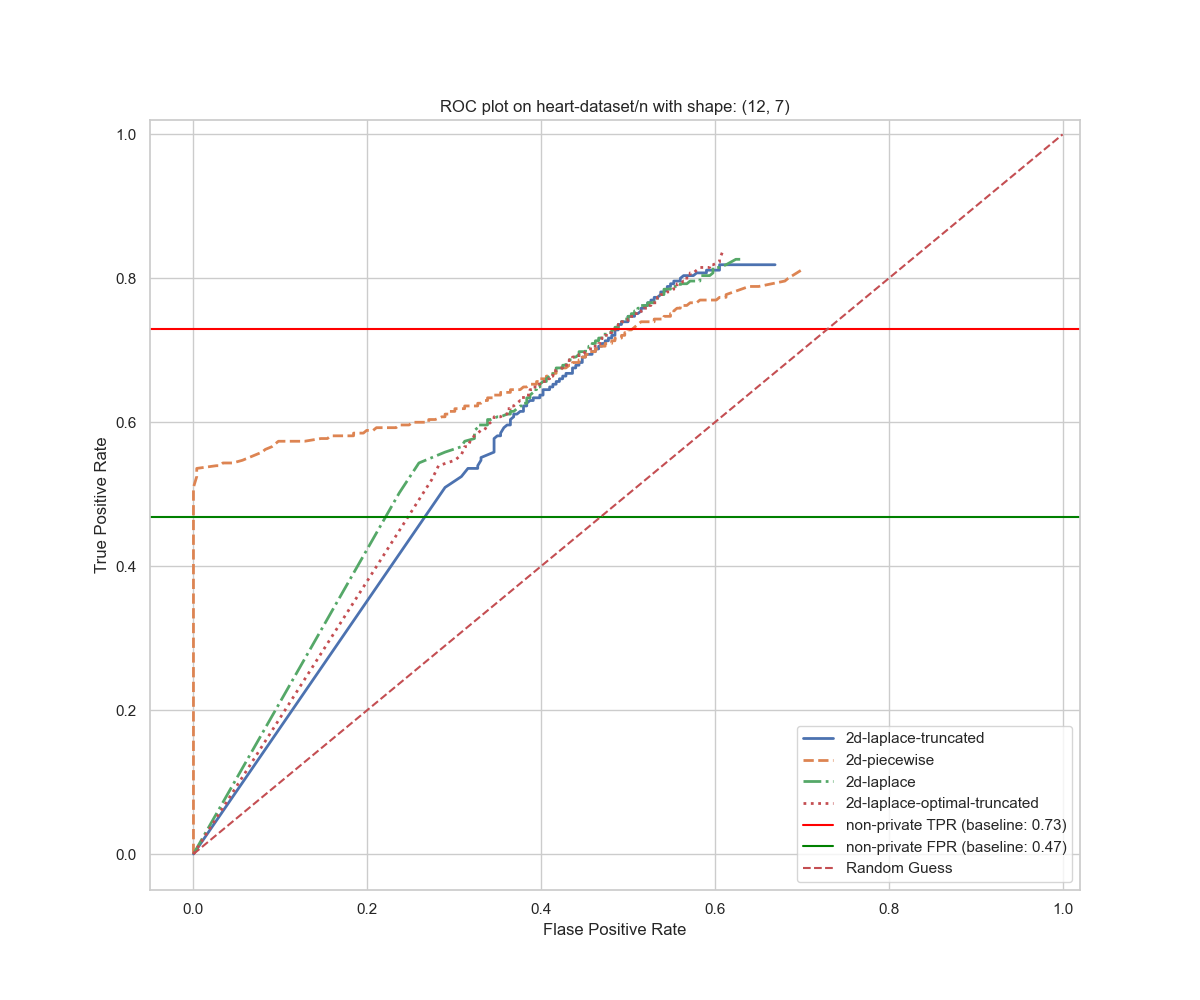
\includegraphics[width=1\textwidth]{Results/RQ1/heart-dataset/roc_plot.png}
        \caption{ROC-curve for privacy per privacy mechanism for heart-dataset.}
        \label{fig:privacy_heart-dataset_comparison_2d_roc_plot}
    \end{minipage}
\end{figure}

\begin{tabular}{llrr}
\toprule
 &  & True Positive Rate & False Positive Rate \\
algorithm & epsilon &  &  \\
\midrule
\bottomrule
\end{tabular}

\newpage
\begin{table}[H]
    \begin{tabularx}{.8\textwidth}{llrr}
        \toprule
                                  &         & True Positive Rate & False Positive Rate \\
        algorithm                 & epsilon &                    &                     \\
        \midrule
        laplace                   & 0.1     & 0.684              & 0.170               \\
                                  & 0.5     & 0.698              & 0.387               \\
        laplace-optimal-truncated & 1.0     & 0.695              & 0.483               \\
        laplace-truncated         & 5.0     & 0.705              & 0.594               \\
        piecewise                 & 0.5     & 0.694              & 0.117               \\
                                  & 0.7     & 0.688              & 0.140               \\
                                  & 1.5     & 0.688              & 0.245               \\
                                  & 2.0     & 0.697              & 0.315               \\
                                  & 2.5     & 0.704              & 0.231               \\
                                  & 3.0     & 0.711              & 0.234               \\
                                  & 3.5     & 0.700              & 0.249               \\
                                  & 7.0     & 0.702              & 0.242               \\
                                  & 9.0     & 0.717              & 0.249               \\
        \bottomrule
    \end{tabularx}
    \caption{Mean privacy scores that are outside specification for the TPR (non-private baseline) for seeds dataset (\ref{fig:privacy_seeds-dataset_comparison_2d_roc_plot})}

\end{table}


\begin{figure}[H]
    \centering
    \begin{minipage}[c]{0.90\textwidth}
        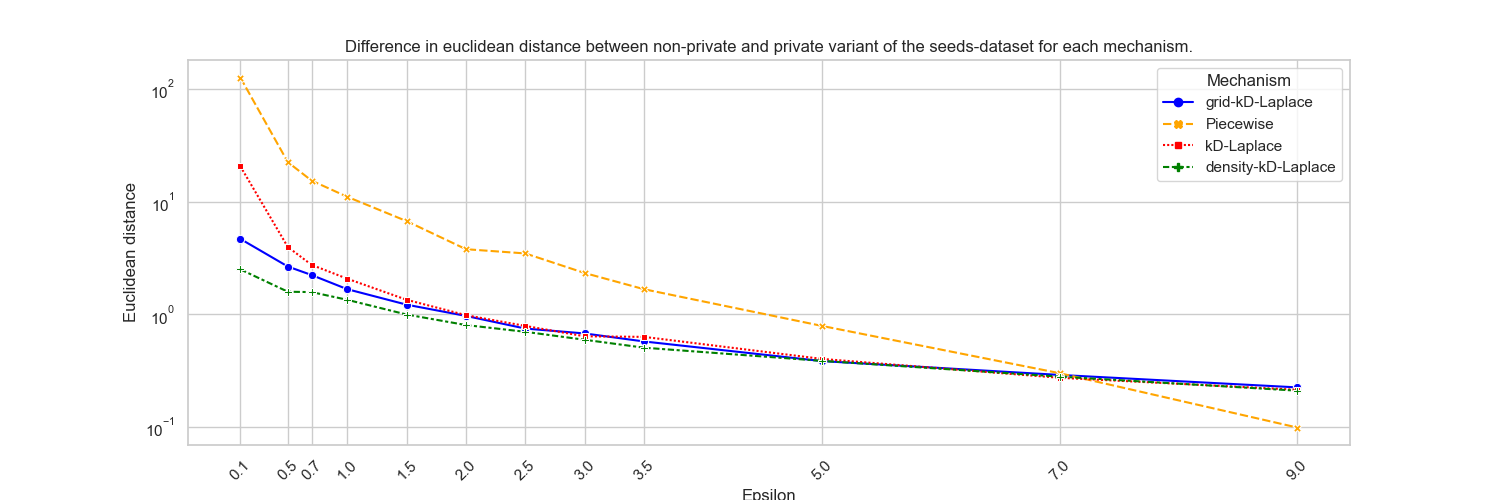
\includegraphics[width=1\textwidth]{Results/RQ1/seeds-dataset/privacy_distance_plot.png}
        \caption{Privacy distance for each mechanism for seeds-dataset.}
        \label{fig:privacy_seeds-dataset_comparison_2d_privacy_distance_plot}
    \end{minipage}
    \begin{minipage}[c]{0.90\textwidth}
        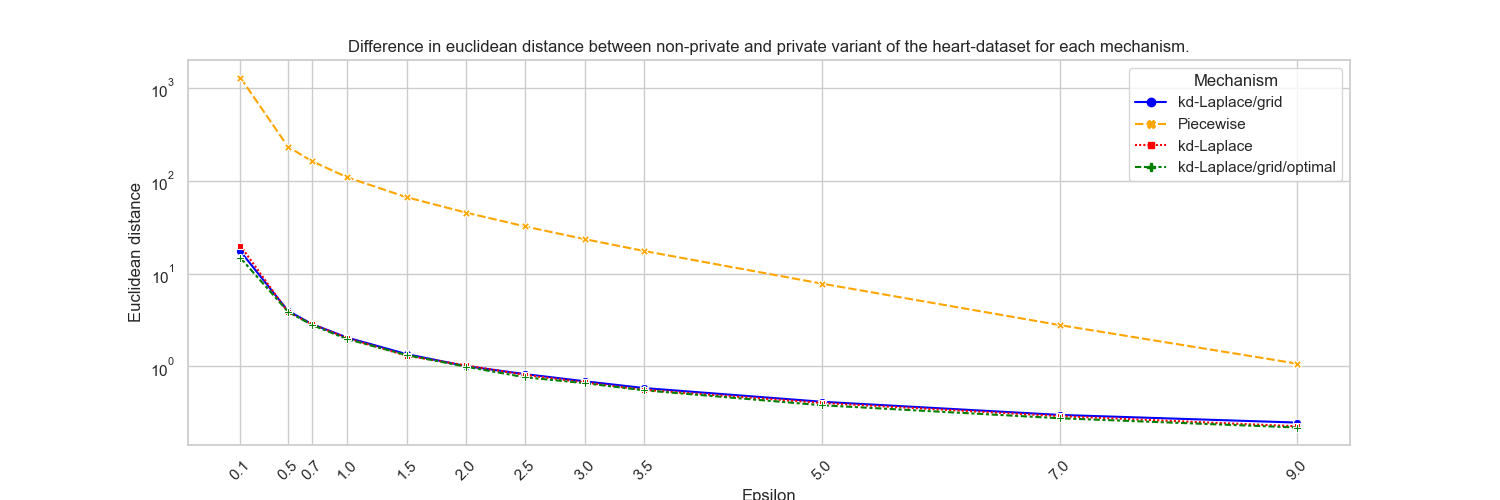
\includegraphics[width=1\textwidth]{Results/RQ1/heart-dataset/privacy_distance_plot.png}
        \caption{Privacy distance for each mechanism for heart-dataset.}
        \label{fig:privacy_heart-dataset_comparison_2d_privacy_distance_plot}
    \end{minipage}
\end{figure}

\newpage
\subsection{3-dimensional data}
\begin{figure}[H]
    \centering
    \begin{minipage}[c]{0.49\textwidth}
        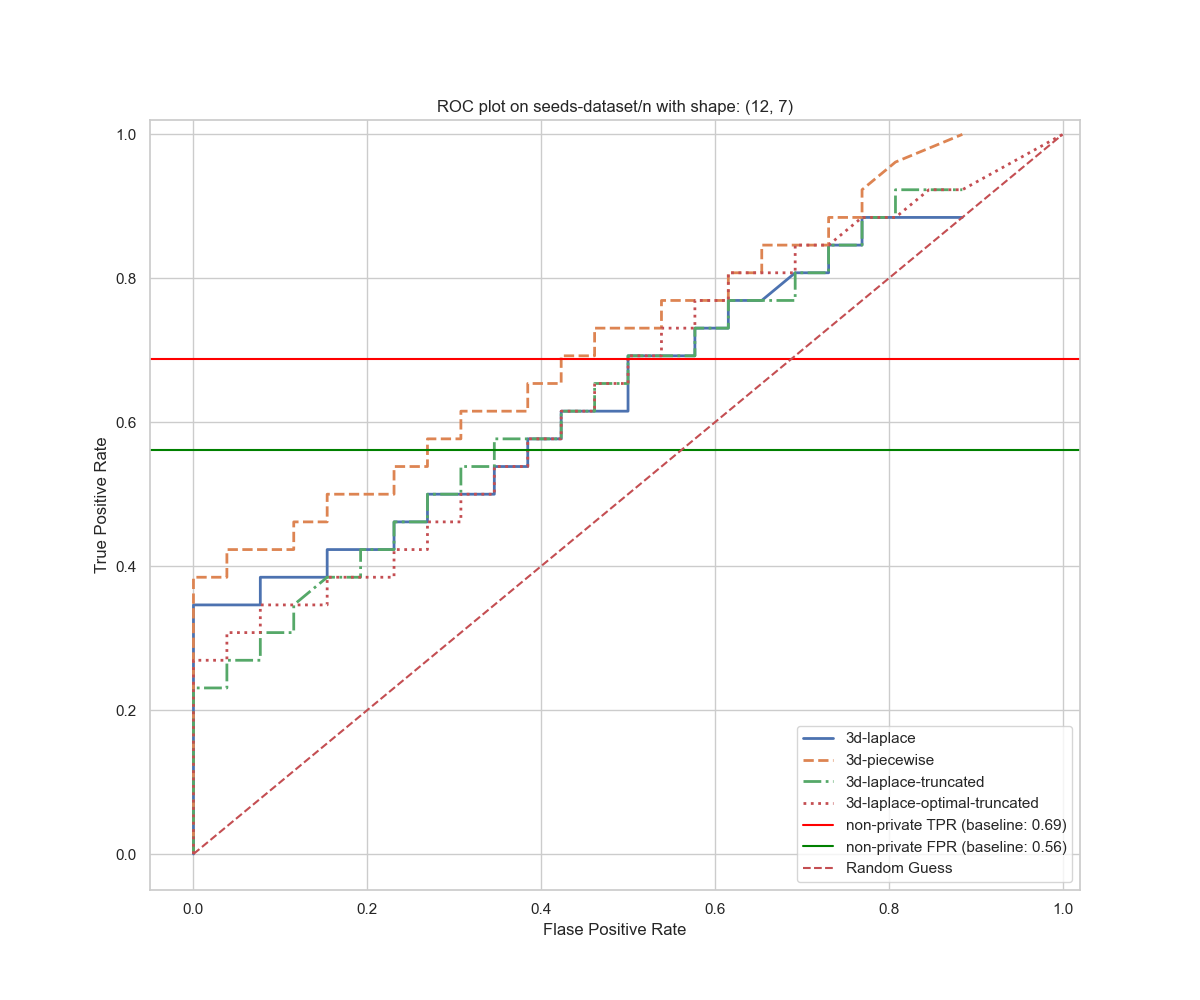
\includegraphics[width=1\textwidth]{Results/RQ2/seeds-dataset/roc_plot.png}
        \caption{ROC-curve for privacy per privacy mechanism for 3-dimensional seeds-dataset.}
        \label{fig:privacy_seeds-dataset_comparison_3d_roc_plot}
    \end{minipage}
    \begin{minipage}[c]{0.49\textwidth}
        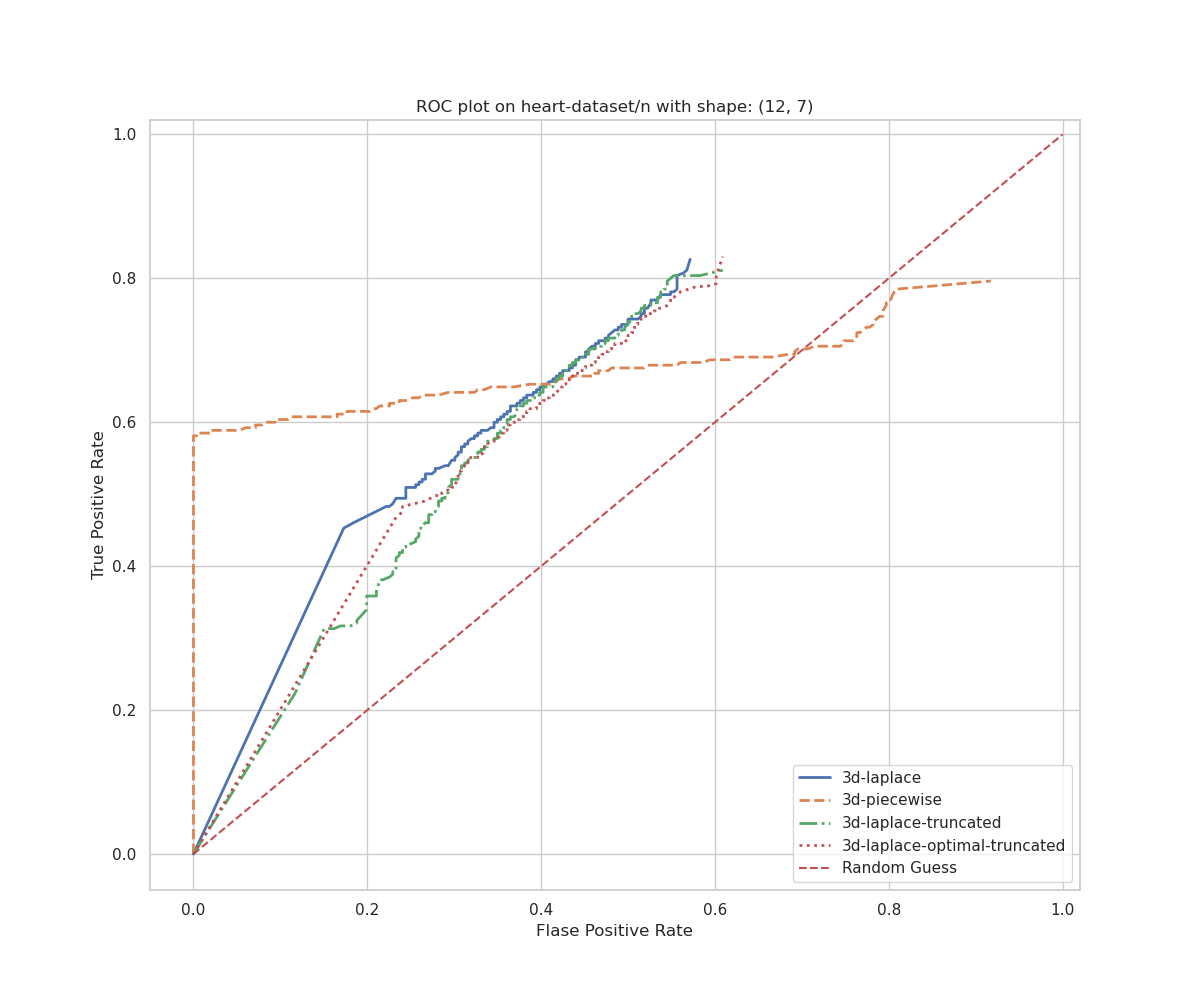
\includegraphics[width=1\textwidth]{Results/RQ2/heart-dataset/roc_plot.png}
        \caption{ROC-curve for privacy per privacy mechanism for 3-dimensional heart-dataset.}
        \label{fig:privacy_heart-dataset_comparison_3d_roc_plot}
    \end{minipage}
\end{figure}

\begin{figure}[H]
    \centering
    \begin{minipage}[c]{0.70\textwidth}
        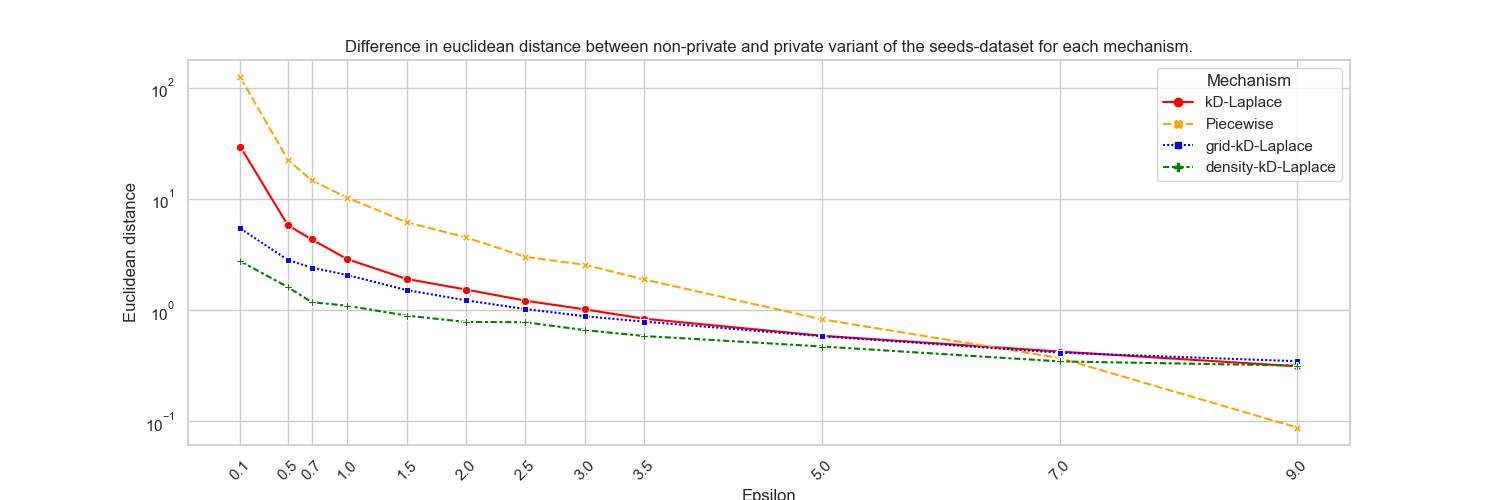
\includegraphics[width=1\textwidth]{Results/RQ2/seeds-dataset/privacy_distance_plot.png}
        \caption{Privacy distance for each mechanism for 3D seeds-dataset.}
        \label{fig:privacy_seeds-dataset_comparison_3d_privacy_distance_plot}
    \end{minipage}
    \begin{minipage}[c]{0.70\textwidth}
        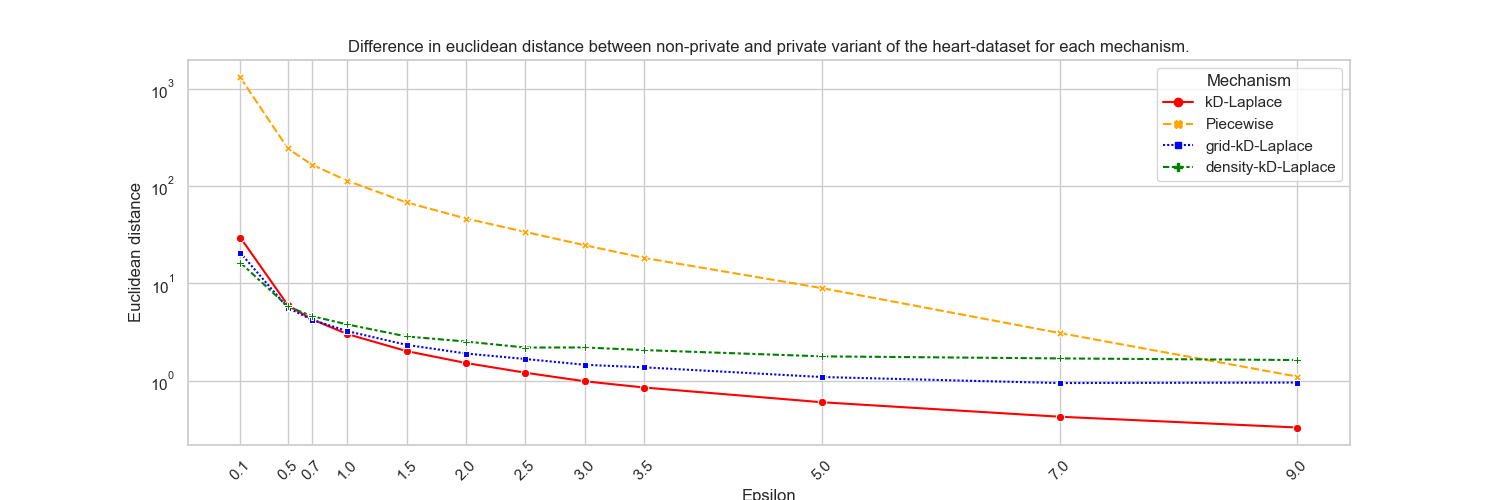
\includegraphics[width=1\textwidth]{Results/RQ2/heart-dataset/privacy_distance_plot.png}
        \caption{Privacy distance for each mechanism for 3D heart-dataset.}
        \label{fig:privacy_heart-dataset_comparison_3d_privacy_distance_plot}
    \end{minipage}
\end{figure}
\begin{tabular}{llrr}
\toprule
\bottomrule
\end{tabular}

\begin{table}[H]
    \begin{tabularx}{0.8\textwidth}{llrr}
        \toprule
                                  &         & True Positive Rate & False Positive Rate \\
        algorithm                 & epsilon &                    &                     \\
        \midrule
        laplace-optimal-truncated & 1.5     & 0.675              & 0.470               \\
                                  & 2.0     & 0.647              & 0.478               \\
                                  & 3.5     & 0.644              & 0.515               \\
                                  & 5.0     & 0.669              & 0.499               \\
        piecewise                 & 7.0     & 0.678              & 0.266               \\
                                  & 9.0     & 0.678              & 0.255               \\
        \bottomrule
    \end{tabularx}
    \caption{Mean privacy scores that are outside specification for the TPR (non-private baseline) for seeds dataset (\ref{fig:privacy_seeds-dataset_comparison_3d_roc_plot})}

\end{table}
\newpage
%\subsection{Utility}
%subsubsection*{Cluster comparison}
%\todo[inline]{Add plot}
%\subsubsection*{Mechanism comparison}
%\begin{figure}[H]
%    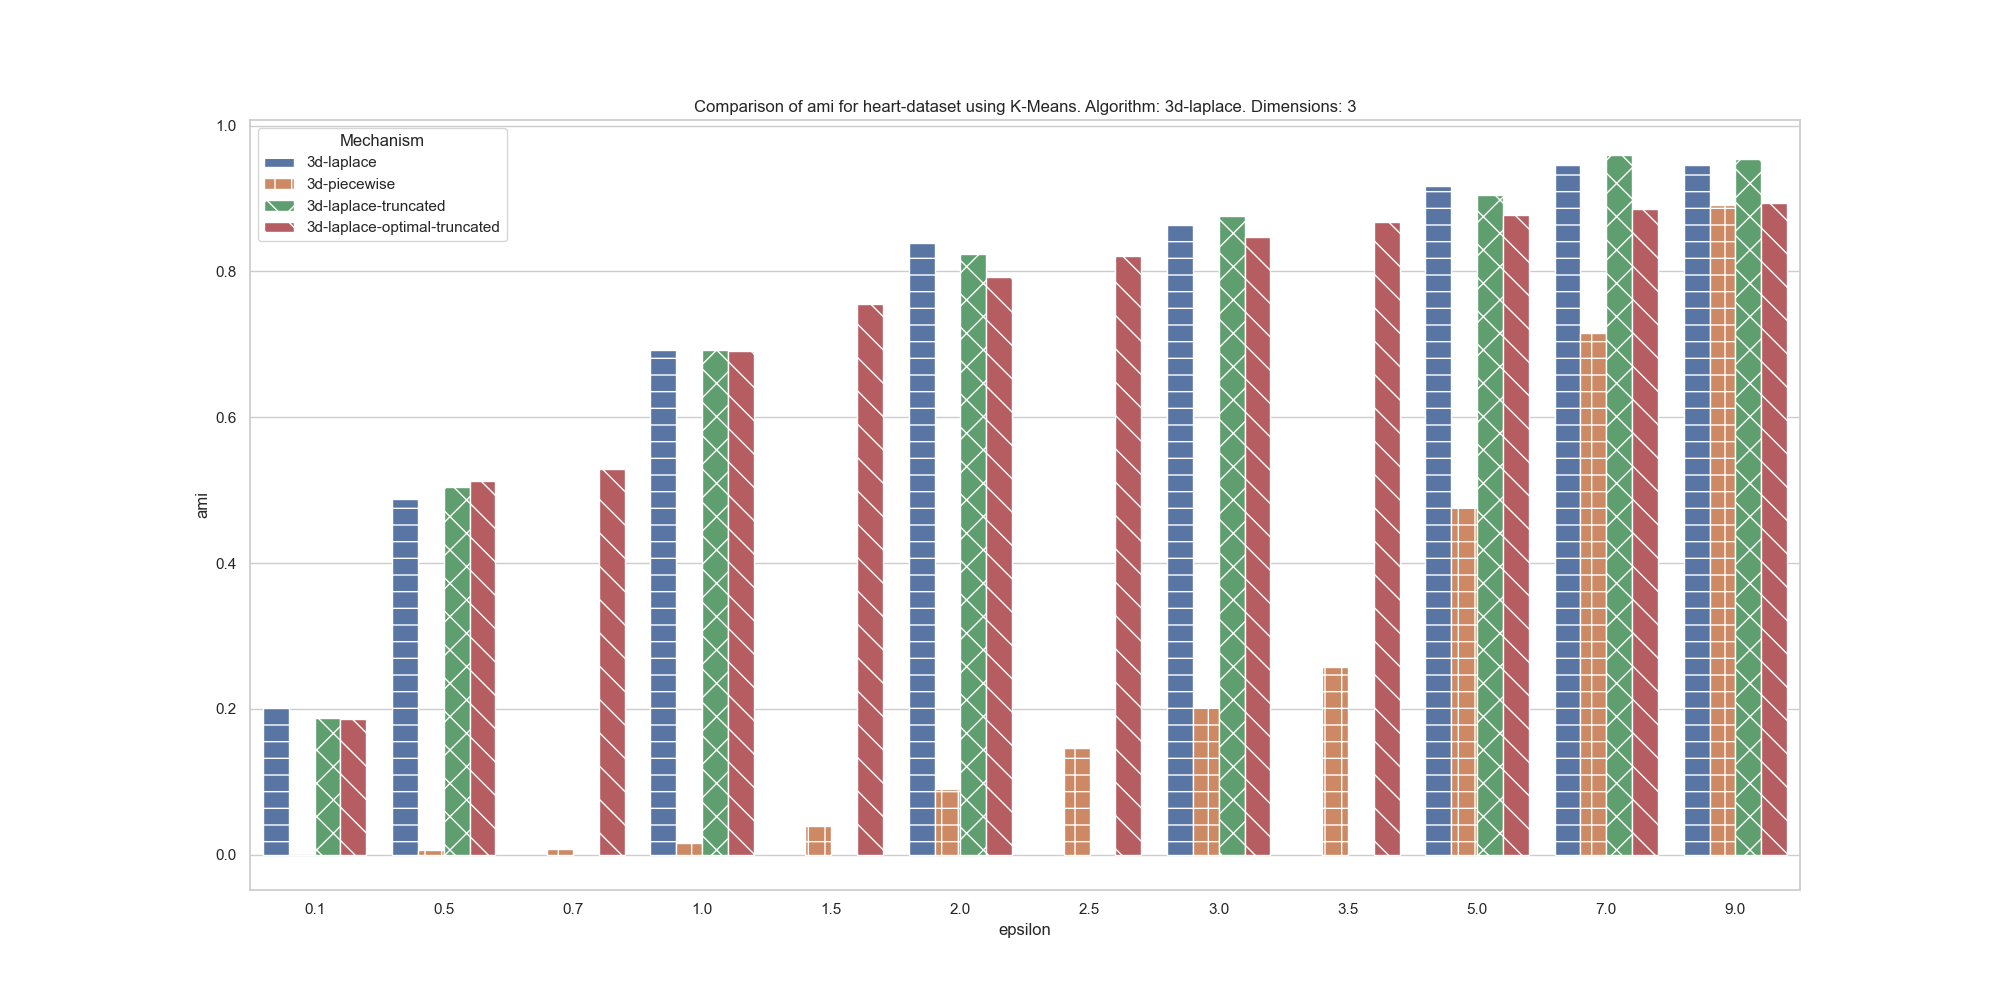
\includegraphics[width=\textwidth]{Results/RQ2/heart-dataset/ami_heart-dataset_comparison.png}
%    \caption{Adjusted Mutual Information comparison for the 3-dimensional heart-dataset}
%    \label{fig:ami_heart-dataset_comparison_3d}
%\end{figure}
%\begin{figure}[H]
%    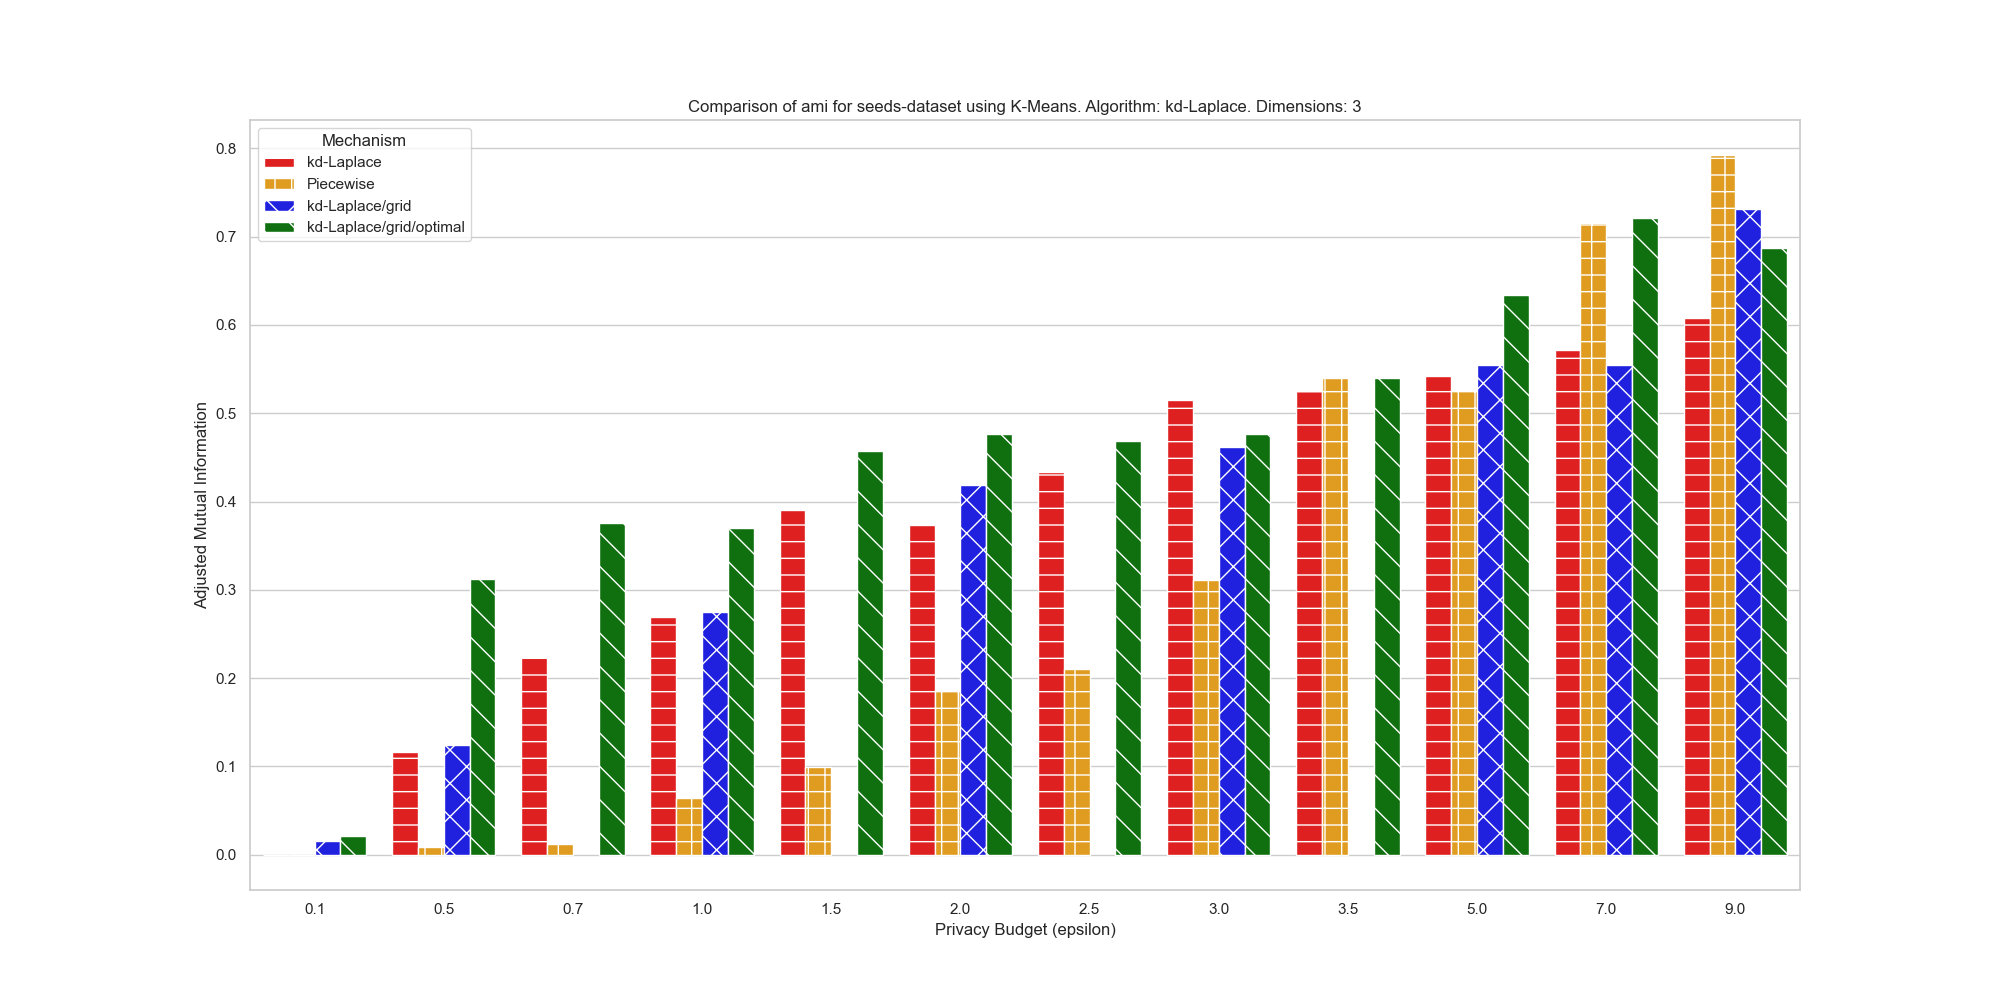
\includegraphics[width=\textwidth]{Results/RQ2/seeds-dataset/ami_seeds-dataset_comparison.png}
%    \caption{Adjusted Mutual Information comparison for the 3-dimensional seeds-dataset}
%    \label{fig:ami_seeds-dataset_comparison_3d}
%\end{figure}
%\todo[inline]{Add links to scilliouette plots and other plots}
\subsection{n-dimensional data}
\begin{figure}[H]
    \centering
    \begin{minipage}[c]{0.49\textwidth}
        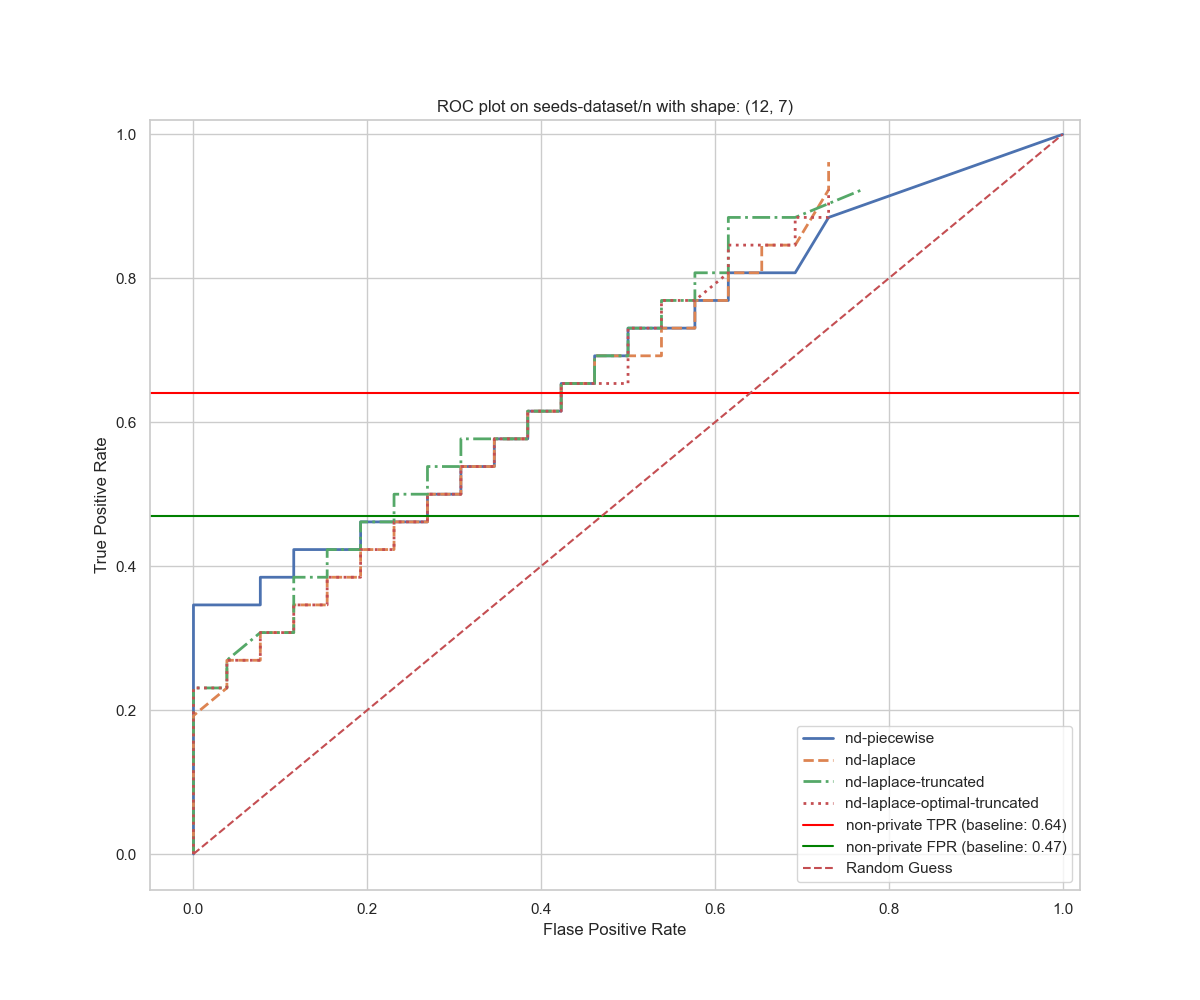
\includegraphics[width=1\textwidth]{Results/RQ2-nd/seeds-dataset/roc_plot.png}
        \caption{ROC-curve for privacy per privacy mechanism for n-dimensional seeds-dataset.}
        \label{fig:privacy_seeds-dataset_comparison_nd_roc_plot}
    \end{minipage}
    \begin{minipage}[c]{0.49\textwidth}
        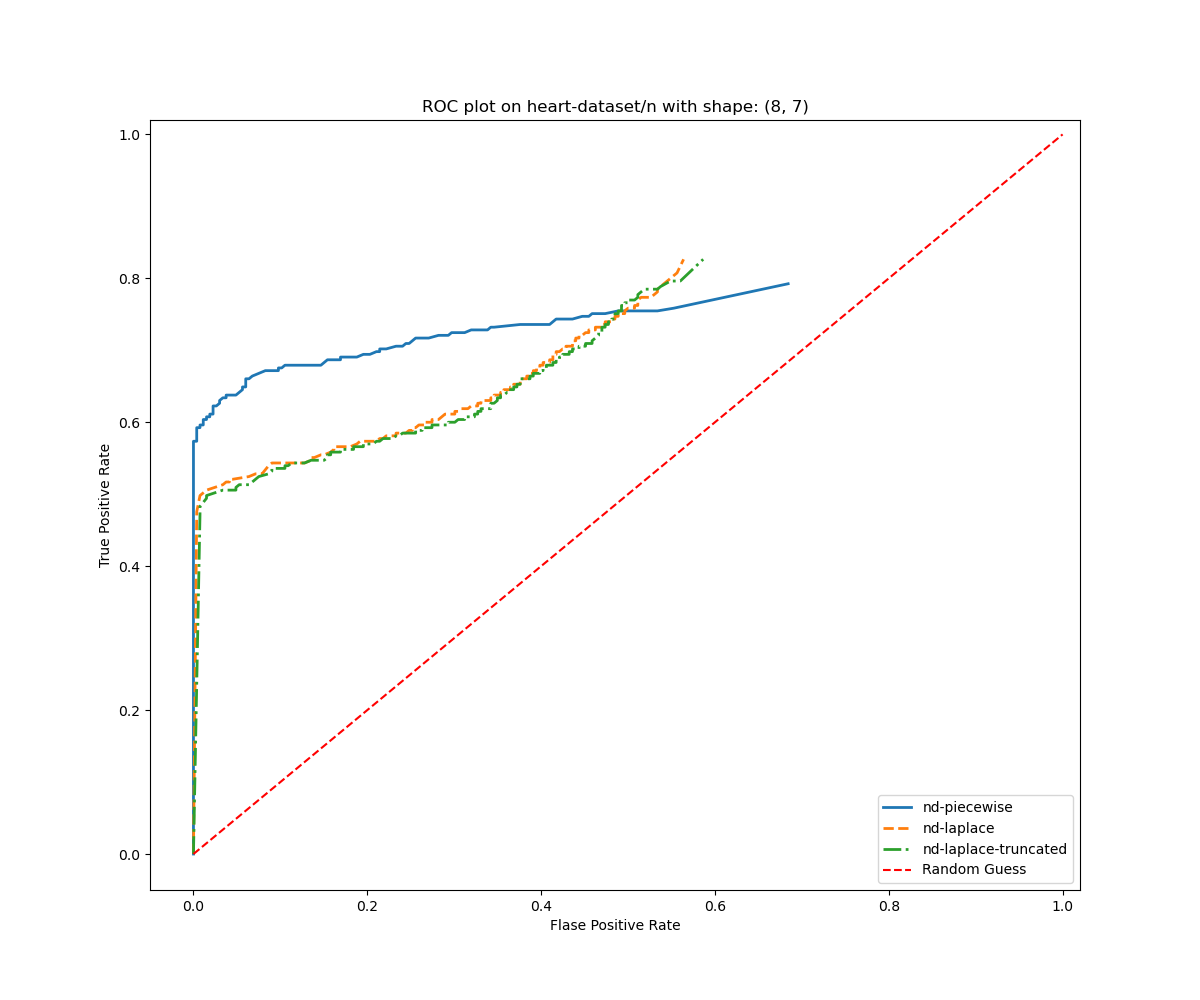
\includegraphics[width=1\textwidth]{Results/RQ2-nd/heart-dataset/roc_plot.png}
        \caption{ROC-curve for privacy per privacy mechanism for n-dimensional heart-dataset.}
        \label{fig:privacy_heart-dataset_comparison_nd_roc_plot}
    \end{minipage}
\end{figure}


%\begin{tabular}{llrr}
\toprule
 &  & True Positive Rate & False Positive Rate \\
algorithm & epsilon &  &  \\
\midrule
\bottomrule
\end{tabular}

\begin{tabular}{llrr}
\toprule
 &  & True Positive Rate & False Positive Rate \\
algorithm & epsilon &  &  \\
\midrule
laplace-truncated & 7.000000 & 0.642000 & 0.418000 \\
\cline{1-4}
\bottomrule
\end{tabular}


\begin{figure}[H]
    \centering
    \begin{minipage}[c]{0.80\textwidth}
        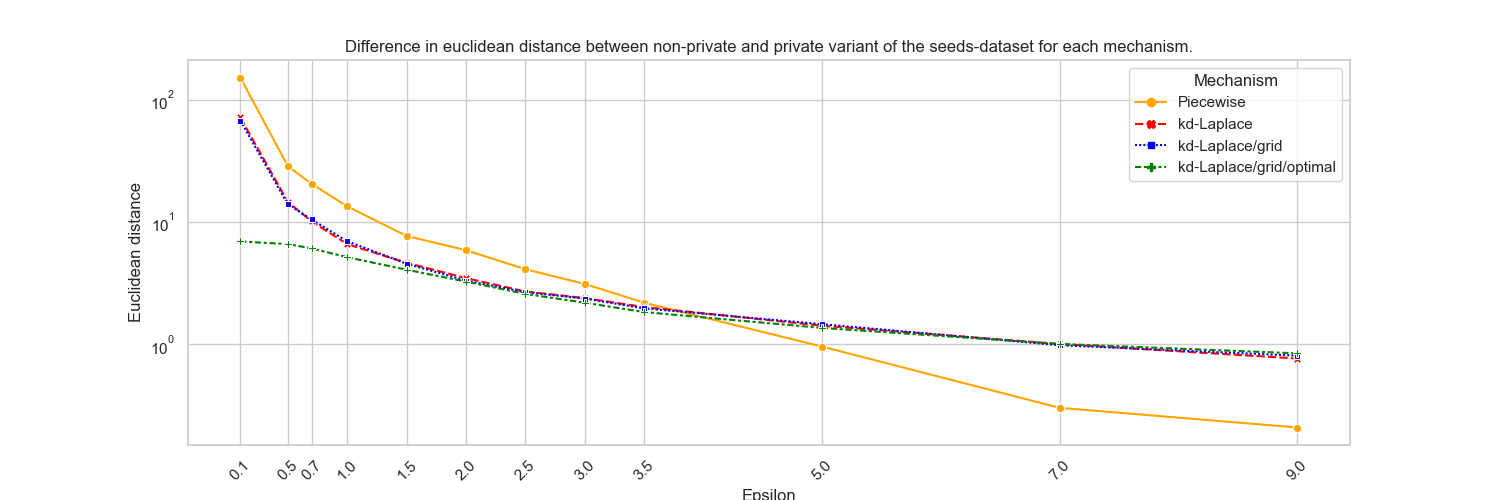
\includegraphics[width=1\textwidth]{Results/RQ2-nd/seeds-dataset/privacy_distance_plot.png}
        \caption{Privacy distance for each mechanism for nD seeds-dataset.}
        \label{fig:privacy_seeds-dataset_comparison_nd_privacy_distance_plot}
    \end{minipage}
    \begin{minipage}[c]{0.80\textwidth}
        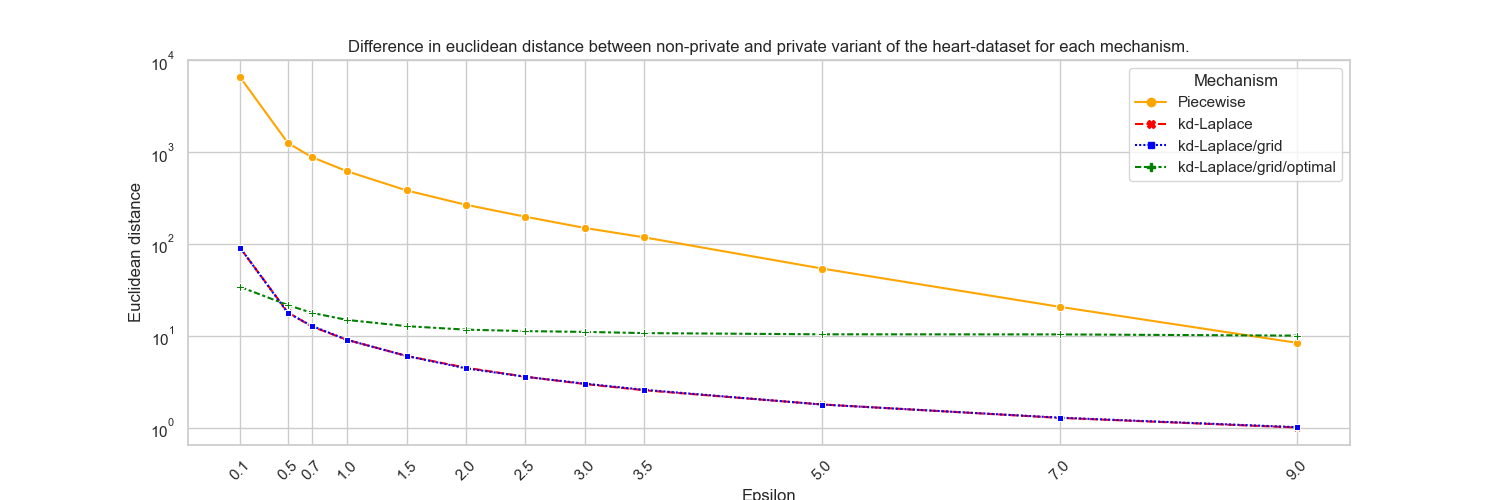
\includegraphics[width=1\textwidth]{Results/RQ2-nd/heart-dataset/privacy_distance_plot.png}
        \caption{Privacy distance for each mechanism for nD heart-dataset.}
        \label{fig:privacy_heart-dataset_comparison_nd_privacy_distance_plot}
    \end{minipage}
\end{figure}

\newpage
\section{Dimensionality}
\todo[inline]{Work in progress}